% Lines starting with a percent sign (%) are comments. LaTeX will 
% not process those lines. Similarly, everything after a percent 
% sign in a line is considered a comment. To produce a percent sign
% in the output, write \% (backslash followed by the percent sign). 
% ==================================================================
% Usage instructions:
% ------------------------------------------------------------------
% The file is heavily commented so that you know what the various
% commands do. Feel free to remove any comments you don't need from
% your own copy. When redistributing the example thesis file, please
% retain all the comments for the benefit of other thesis writers! 
% ==================================================================
% Compilation instructions: 
% ------------------------------------------------------------------
% Use pdflatex to compile! Input images are expected as PDF files.
% Example compilation:
% ------------------------------------------------------------------
% > pdflatex thesis-example.tex
% > bibtex thesis-example
% > pdflatex thesis-example.tex
% > pdflatex thesis-example.tex
% ------------------------------------------------------------------
% You need to run pdflatex multiple times so that all the cross-references
% are fixed. pdflatex will tell you if you need to re-run it (a warning
% will be issued)  
% ------------------------------------------------------------------
% Compilation has been tested to work in ukk.cs.hut.fi and kosh.hut.fi
% - if you have problems of missing .sty -files, then the local LaTeX
% environment does not have all the required packages installed.
% For example, when compiling in vipunen.hut.fi, you get an error that
% tikz.sty is missing - in this case you must either compile somewhere
% else, or you cannot use TikZ graphics in your thesis and must therefore
% remove or comment out the tikz package and all the tikz definitions. 
% ------------------------------------------------------------------

% General information
% ==================================================================
% Package documentation:
% 
% The comments often refer to package documentation. (Almost) all LaTeX
% packages have documentation accompanying them, so you can read the
% package documentation for further information. When a package 'xxx' is
% installed to your local LaTeX environment (the document compiles
% when you have \usepackage{xxx} and LaTeX does not complain), you can 
% find the documentation somewhere in the local LaTeX texmf directory
% hierarchy. In ukk.cs.hut.fi, this is /usr/texlive/2008/texmf-dist,
% and the documentation for the titlesec package (for example) can be 
% found at /usr/texlive/2008/texmf-dist/doc/latex/titlesec/titlesec.pdf.
% Most often the documentation is located as a PDF file in 
% /usr/texlive/2008/texmf-dist/doc/latex/xxx, where xxx is the package name; 
% however, documentation for TikZ is in
% /usr/texlive/2008/texmf-dist/doc/latex/generic/pgf/pgfmanual.pdf
% (this is because TikZ is a front-end for PGF, which is meant to be a 
% generic portable graphics format for LaTeX).
% You can try to look for the package manual using the ``find'' shell
% command in Linux machines; the find databases are up-to-date at least
% in ukk.cs.hut.fi. Just type ``find xxx'', where xxx is the package
% name, and you should find a documentation file.
% Note that in some packages, the documentation is in the DVI file
% format. In this case, you can copy the DVI file to your home directory,
% and convert it to PDF with the dvipdfm command (or you can read the
% DVI file directly with a DVI viewer).
% 
% If you can't find the documentation for a package, just try Googling
% for ``latex packagename''; most often you can get a direct link to the
% package manual in PDF format.
% ------------------------------------------------------------------


% Document class for the thesis is report
% ------------------------------------------------------------------
% You can change this but do so at your own risk - it may break other things.
% Note that the option pdftext is used for pdflatex; there is no
% pdflatex option. 
% ------------------------------------------------------------------
\documentclass[12pt,a4paper,oneside,pdftex]{report}

% The input files (tex files) are encoded with the latin-1 encoding 
% (ISO-8859-1 works). Change the latin1-option if you use UTF8 
% (at some point LaTeX did not work with UTF8, but I'm not sure
% what the current situation is) 
\usepackage[utf8]{inputenc}
% OT1 font encoding seems to work better than T1. Check the rendered
% PDF file to see if the fonts are encoded properly as vectors (instead
% of rendered bitmaps). You can do this by zooming very close to any letter 
% - if the letter is shown pixelated, you should change this setting 
% (try commenting out the entire line, for example).  
\usepackage[OT1]{fontenc}
% The babel package provides hyphenating instructions for LaTeX. Give
% the languages you wish to use in your thesis as options to the babel
% package (as shown below). You can remove any language you are not
% going to use.
% Examples of valid language codes: english (or USenglish), british, 
% finnish, swedish; and so on.
\usepackage[finnish,swedish,english]{babel}


% Font selection
% ------------------------------------------------------------------
% The default LaTeX font is a very good font for rendering your 
% thesis. It is a very professional font, which will always be 
% accepted. 
% If you, however, wish to spicen up your thesis, you can try out
% these font variants by uncommenting one of the following lines
% (or by finding another font package). The fonts shown here are 
% all fonts that you could use in your thesis (not too silly). 
% Changing the font causes the layouts to shift a bit; you many
% need to manually adjust some layouts. Check the warning messages
% LaTeX gives you.
% ------------------------------------------------------------------
% To find another font, check out the font catalogue from
% http://www.tug.dk/FontCatalogue/mathfonts.html
% This link points to the list of fonts that support maths, but
% that's a fairly important point for master's theses.
% ------------------------------------------------------------------
% <rant>
% Remember, there is no excuse to use Comic Sans, ever, in any
% situation! (Well, maybe in speech bubbles in comics, but there 
% are better options for those too)
% </rant>

% \usepackage{palatino}
% \usepackage{tgpagella}



% Optional packages
% ------------------------------------------------------------------
% Select those packages that you need for your thesis. You may delete
% or comment the rest.

% Natbib allows you to select the format of the bibliography references.
% The first example uses numbered citations: 
\usepackage[square,sort&compress,numbers]{natbib}
% The second example uses author-year citations.
% If you use author-year citations, change the bibliography style (below); 
% acm style does not work with author-year citations.
% Also, you should use \citet (cite in text) when you wish to refer
% to the author directly (\citet{blaablaa} said blaa blaa), and 
% \citep when you wish to refer similarly than with numbered citations
% (It has been said that blaa blaa~\citep{blaablaa}).
% \usepackage[square]{natbib}

% The alltt package provides an all-teletype environment that acts
% like verbatim but you can use LaTeX commands in it. Uncomment if 
% you want to use this environment. 
% \usepackage{alltt}

% The eurosym package provides a euro symbol. Use with \euro{}
\usepackage{eurosym} 

% Verbatim provides a standard teletype environment that renderes
% the text exactly as written in the tex file. Useful for code
% snippets (although you can also use the listings package to get
% automatic code formatting). 
\usepackage{verbatim}

% The listing package provides automatic code formatting utilities
% so that you can copy-paste code examples and have them rendered
% nicely. See the package documentation for details.
% \usepackage{listings}

% The fancuvrb package provides fancier verbatim environments 
% (you can, for example, put borders around the verbatim text area
% and so on). See package for details.
% \usepackage{fancyvrb}

% Supertabular provides a tabular environment that can span multiple 
% pages. 
%\usepackage{supertabular}
% Longtable provides a tabular environment that can span multiple 
% pages. This is used in the example acronyms file. 
\usepackage{longtable}
\usepackage{threeparttable}
\usepackage[skip=8pt]{caption}

% The fancyhdr package allows you to set your the page headers 
% manually, and allows you to add separator lines and so on. 
% Check the package documentation. 
% \usepackage{fancyhdr}

% Subfigure package allows you to use subfigures (i.e. many subfigures
% within one figure environment). These can have different labels and
% they are numbered automatically. Check the package documentation. 
\usepackage{subfigure}

% The titlesec package can be used to alter the look of the titles 
% of sections, chapters, and so on. This example uses the ``medium'' 
% package option which sets the titles to a medium size, making them
% a bit smaller than what is the default. You can fine-tune the 
% title fonts and sizes by using the package options. See the package
% documentation.
\usepackage[medium]{titlesec}

% The TikZ package allows you to create professional technical figures.
% The learning curve is quite steep, but it is definitely worth it if 
% you wish to have really good-looking technical figures. 
\usepackage{tikz}
% You also need to specify which TikZ libraries you use
\usetikzlibrary{positioning}
\usetikzlibrary{calc}
\usetikzlibrary{arrows}
\usetikzlibrary{decorations.pathmorphing,decorations.markings}
\usetikzlibrary{shapes}
\usetikzlibrary{patterns}


% The aalto-thesis package provides typesetting instructions for the
% standard master's thesis parts (abstracts, front page, and so on)
% Load this package second-to-last, just before the hyperref package.
% Options that you can use: 
%   mydraft - renders the thesis in draft mode. 
%             Do not use for the final version. 
%   doublenumbering - [optional] number the first pages of the thesis
%                     with roman numerals (i, ii, iii, ...); and start
%                     arabic numbering (1, 2, 3, ...) only on the 
%                     first page of the first chapter
%   twoinstructors  - changes the title of instructors to plural form
%   twosupervisors  - changes the title of supervisors to plural form
\usepackage[mydraft]{aalto-thesis}
%\usepackage[mydraft,doublenumbering]{aalto-thesis}
%\usepackage{aalto-thesis}



% Hyperref
% ------------------------------------------------------------------
% Hyperref creates links from URLs, for references, and creates a
% TOC in the PDF file.
% This package must be the last one you include, because it has
% compatibility issues with many other packages and it fixes
% those issues when it is loaded.   
%\RequirePackage[pdftex]{hyperref}
\RequirePackage[pdfa]{hyperref}
% Setup hyperref so that links are clickable but do not look 
% different
\hypersetup{colorlinks=false,raiselinks=false,breaklinks=true}
\hypersetup{pdfborder={0 0 0}}
\hypersetup{bookmarksnumbered=true}
% The following line suggests the PDF reader that it should show the 
% first level of bookmarks opened in the hierarchical bookmark view. 
\hypersetup{bookmarksopen=true,bookmarksopenlevel=1}
% Hyperref can also set up the PDF metadata fields. These are
% set a bit later on, after the thesis setup.   


% Thesis setup
% ==================================================================
% Change these to fit your own thesis.
% \COMMAND always refers to the English version;
% \FCOMMAND refers to the Finnish version; and
% \SCOMMAND refers to the Swedish version.
% You may comment/remove those language variants that you do not use
% (but then you must not include the abstracts for that language)
% ------------------------------------------------------------------
% If you do not find the command for a text that is shown in the cover page or
% in the abstract texts, check the aalto-thesis.sty file and locate the text
% from there. 
% All the texts are configured in language-specific blocks (lots of commands
% that look like this: \renewcommand{\ATCITY}{Espoo}.
% You can just fix the texts there. Just remember to check all the language
% variants you use (they are all there in the same place). 
% ------------------------------------------------------------------
\newcommand{\TITLE}{Engineering analytics of big data pipelines for stock market data}
\newcommand{\FTITLE}{Osakemarkkina dataa käsittelevien big data järjestelmien tekninen analyysi}
%\newcommand{\STITLE}{Den stora stygga vargen:}
\newcommand{\SUBTITLE}{}
\newcommand{\FSUBTITLE}{}
%\newcommand{\SSUBTITLE}{Lilla Vargens universum}
\newcommand{\DATE}{October 9, 2019}
\newcommand{\FDATE}{9. lokakuuta 2019}
%\newcommand{\SDATE}{Den 18 februari 2018}

% Supervisors and instructors
% ------------------------------------------------------------------
% Usually thesis have one supervisor and one advisor. Sometimes you
% may have two advisors and, in double degree
% programs, you may have two supervisors. 
% If you have two supervisors, write both names here, separate them with a 
% double-backslash (see below for an example)
% Also remember to add the package option ``twosupervisors'' or
% ``twoinstructors'' to the aalto-thesis package (aalto-thesis.sty
% file line 72), so that the titles are in plural.
% Example of one supervisor:
%\newcommand{\SUPERVISOR}{Professor Antti Yl�-J��ski}
%\newcommand{\FSUPERVISOR}{Professori Antti Yl�-J��ski}
%\newcommand{\SSUPERVISOR}{Professor Antti Yl�-J��ski}
% Example of twosupervisors:
\newcommand{\SUPERVISOR}{Professor Linh Truong}
\newcommand{\FSUPERVISOR}{Professori Linh Truong}
%\newcommand{\SSUPERVISOR}{Professor Antti Yl�-J��ski\\
 % Professor Petra Perustieteilij�}

% If you have only one instructor, just write one name here
\newcommand{\INSTRUCTOR}{Professor Linh Truong}
\newcommand{\FINSTRUCTOR}{Professori Linh Truong}
%\newcommand{\SINSTRUCTOR}{Diplomingenj�r Oili Ohjaaja}
% If you have two instructors, separate them with \\ to create linefeeds
% \newcommand{\INSTRUCTOR}{Oili Ohjaaja M.Sc. (Tech.)\\
%  Elli Opas M.Sc. (Tech)}
%\newcommand{\FINSTRUCTOR}{Diplomi-insin��ri Oili Ohjaaja\\
%  Diplomi-insin��ri Elli Opas}
%\newcommand{\SINSTRUCTOR}{Diplomingenj�r Oili Ohjaaja\\
%  Diplomingenj�r Elli Opas}

% If you have two supervisors, it is common to write the schools
% of the supervisors in the cover page. If the following command is defined,
% then the supervisor names shown here are printed in the cover page. Otherwise,
% the supervisor names defined above are used.
%\newcommand{\COVERSUPERVISOR}{Professor Antti Yl�-J��ski, Aalto University\\
  %Professor Petra Perustieteilij�, University of Helsinki}

% The same option is for the instructors, if you have multiple instructors.
% \newcommand{\COVERINSTRUCTOR}{Oili Ohjaaja M.Sc. (Tech.), Aalto University\\
%  Elli Opas M.Sc. (Tech), Aalto SCI}


% Other stuff
% ------------------------------------------------------------------
\newcommand{\PROFESSORSHIP}{Computer Science}
\newcommand{\FPROFESSORSHIP}{Tietotekniikka}
%\newcommand{\SPROFESSORSHIP}{Datateknik}
% Professorship code is the same in all languages
\newcommand{\PROFCODE}{SCI3042}
\newcommand{\KEYWORDS}{stock market, big data, cloud computing, data analysis}
\newcommand{\FKEYWORDS}{osakkeet, big data, pilvilaskenta}
%\newcommand{\SKEYWORDS}{oms�ttning, kassafl�de, v�rdepappersmarknadslagen,
%yrkesut�vare, intressef�retag, verifieringskedja}
\newcommand{\LANGUAGE}{English}
\newcommand{\FLANGUAGE}{Englanti}
%\newcommand{\SLANGUAGE}{Engelska}

% Author is the same for all languages
\newcommand{\AUTHOR}{Ville Vainio}


% Currently the English versions are used for the PDF file metadata
% Set the PDF title
\hypersetup{pdftitle={\TITLE\ \SUBTITLE}}
% Set the PDF author
\hypersetup{pdfauthor={\AUTHOR}}
% Set the PDF keywords
\hypersetup{pdfkeywords={\KEYWORDS}}
% Set the PDF subject
\hypersetup{pdfsubject={Master's Thesis}}


% Layout settings
% ------------------------------------------------------------------

% When you write in English, you should use the standard LaTeX 
% paragraph formatting: paragraphs are indented, and there is no 
% space between paragraphs.
% When writing in Finnish, we often use no indentation in the
% beginning of the paragraph, and there is some space between the 
% paragraphs. 

% If you write your thesis Finnish, uncomment these lines; if 
% you write in English, leave these lines commented! 
% \setlength{\parindent}{0pt}
% \setlength{\parskip}{1ex}

% Use this to control how much space there is between each line of text.
% 1 is normal (no extra space), 1.3 is about one-half more space, and
% 1.6 is about double line spacing.  
% \linespread{1} % This is the default
% \linespread{1.3}

% Bibliography style
% acm style gives you a basic reference style. It works only with numbered
% references.
\bibliographystyle{acm}
% Plainnat is a plain style that works with both numbered and name citations.
% \bibliographystyle{plainnat}


% Extra hyphenation settings
% ------------------------------------------------------------------
% You can list here all the files that are not hyphenated correctly.
% You can provide many \hyphenation commands and/or separate each word
% with a space inside a single command. Put hyphens in the places where
% a word can be hyphenated.
% Note that (by default) LaTeX will not hyphenate words that already
% have a hyphen in them (for example, if you write ``structure-modification 
% operation'', the word structure-modification will never be hyphenated).
% You need a special package to hyphenate those words.
\hyphenation{di-gi-taa-li-sta yksi-suun-tai-sta}



% The preamble ends here, and the document begins. 
% Place all formatting commands and such before this line.
% ------------------------------------------------------------------
\begin{document}
% This command adds a PDF bookmark to the cover page. You may leave
% it out if you don't like it...
\pdfbookmark[0]{Cover page}{bookmark.0.cover}
% This command is defined in aalto-thesis.sty. It controls the page 
% numbering based on whether the doublenumbering option is specified
\startcoverpage

% Cover page
% ------------------------------------------------------------------
% Options: finnish, english, and swedish
% These control in which language the cover-page information is shown
\coverpage{english}


% Abstracts
% ------------------------------------------------------------------
% Include an abstract in the language that the thesis is written in,
% and if your native language is Finnish or Swedish, one in that language.

% Abstract in English
% ------------------------------------------------------------------
\thesisabstract{english}{
The world economics revolve around stock markets.
The information in the stock market does not only represent the current state of economy but it also reflects other phenomenons that affect the prices of the stocks.
This is why there are constantly new academic studies so that we could understand both global economy and these phenomenons better.

The size of the data that the stock market alone produces in a year is in the scale of terabytes.
In order to analyze this data, tools that can handle this much infomation are necessary.
Unfortunately, the information about these tools in the context of stock data is scattered, somewhat outdated and hard to find, which can drive away potential valuable research.
The goal of this thesis is to provide information and tools that can make this analysis more accessible to data analysist.

This thesis performs a literary research on what is the current state of stock data analysis in big data environment focusing on historical data analysis pipelines and based on this research implements an open-source pipeline that anyone can use.
The literary study shows that the current trend in stock data analysis is deep learning models giving the pipelines requirement to support these methods.
In the implementation part we see that running deep learning libraries in distributed enviroment can be quite challenging and provide information about these challenges and how to solve them.
The resulting pipeline does fullfil most of its requirements, but the results of the study are a bit incomplete without better comparative study.

}
%The abstract provides goal, motivation, background, and conclusions of
%the work. It has to fit to one page together with the bibliographical
%information.
% Abstract in Finnish
% ------------------------------------------------------------------

\thesisabstract{finnish}{
Maailman talous pyörii osakemarkkinoiden ympärillä.
Informaatio, jota osakemarkkina tarjoaa ei pelkästään kerro talouden nykytilasta vaan se myös heijastaa kaikkia osakemarkkinoihin vaikuttavia ilmiöitä.
Tämän takia uusia tutkimuksia tehdään jatkuvasti jotta sekä taloutta että näitä ilmiöitä voitaisiin ymmärtää paremmin.

Osakemarkkinoiden tuottaman datan määrä vuodessa on teratavujen mittaluokassa.
Jotta tätä dataa voitaisiin siis tutkia, tarvitaan työkaluja jotka pystyvät toimimaan tämän mittaluokan kanssa.
Valitettavasti informaatio näistä työkaluista osake datan kontekstissa on hajanaista, jossain määrin vanhentunutta ja vaikeasti löydettävissä, mikä jossain tapauksissa estää mahdollisesti tärkeän analysiin tekemisen.
Tämän diplomityön tarkoituksena on tarjota tietoa ja työkaluja, jotta tämän tyyppinen tutkimus olisi mahdollisimman helppopääsyistä tutkijoille, jotka eivät ole tämän alan ammattilaisia.

Tässä diplomityössä suoritamme kirjallisuuskatsauksen tämän hetken osake datan tutkimukseen big data ympäristössä.
Keskitymme historialista dataa käsitteleviin järjestelmiin ja toteutamme avoimen lähdekoodin järjestelmän, jota kuka tahansa voi hyödyntää.
Kirjallisuuskatsaus osoittaa että tämän hetken kehityssuunta osake datan tutkimisessa on deep learning menetelmät, jonka vuoksi järjestelmien on tuettava näitä metodeja.
Työn kokeellisessa osuudessa huomaamme että deep learning ohjelmistokirjastojen käyttö hajautetussa ympäristössä voi olla hyvin hankalaa ja tarjoamme tietoa siitä mitä kaikkea voi mennä vikaan ja miten korjata nämä.
Työn tuloksena saamme kehitettyä järjestelmän joka täyttää suurimman osan sille annetuista vaatimuksista, mutta tulokset jäävät hieman vajaavaisiksi, koska vertailevaa testausta ei ehditä toteuttaa.

}

% Abstract in Swedish
% ------------------------------------------------------------------
%\thesisabstract{swedish}{
%Om ditt skolespr�k �r svenska, m�ste din diplomarbetet  ha en svenskspr�kig sammanfattning. Sammanfattningen m�ste passa p� en sida.}


% Acknowledgements
% ------------------------------------------------------------------
% Select the language you use in your acknowledgements
\selectlanguage{english}

% Uncomment this line if you wish acknoledgements to appear in the 
% table of contents
%\addcontentsline{toc}{chapter}{Acknowledgements}

% The star means that the chapter isn't numbered and does not 
% show up in the TOC
%\chapter*{Acknowledgements}

%I wish to thank all students who use \LaTeX\ for formatting their theses,
%because theses formatted with \LaTeX\ are just so nice.

%Thank you, and keep up the good work!
\vskip 10mm

\noindent Espoo, \DATE
\vskip 5mm
\noindent\AUTHOR

% Acronyms
% ------------------------------------------------------------------
% Use \cleardoublepage so that IF two-sided printing is used 
% (which is not often for masters theses), then the pages will still
% start correctly on the right-hand side.
\cleardoublepage
% Example acronyms are placed in a separate file, acronyms.tex
\addcontentsline{toc}{chapter}{Abbreviations and Acronyms}
\chapter*{Abbreviations and Acronyms}

% The longtable environment should break the table properly to multiple pages, 
% if needed

\noindent
\begin{longtable}{@{}p{0.25\textwidth}p{0.7\textwidth}@{}}
EMH & Efficient Market Hypothesis \\
RSI & Relative Strength Index \\
MACD & Moving Average Convergence Divergence \\
TF-IDF & Term Frequency–Inverse Document Frequency \\
HDFS & Hadoop Distributed File System \\
QoS & Quality of Service \\
DL4J & Deeplearning4j Machine learning library \\
%2k/4k/8k mode & COFDM operation modes \\
%3GPP & 3rd Generation Partnership Project \\ 
%ESP & Encapsulating Security Payload; An IPsec security protocol \\ 
%FLUTE  & The File Delivery over Unidirectional Transport protocol \\ 
%e.g.& for example (do not list here this kind of common acronymbs or abbreviations, but only those that are essential for understanding the content of your thesis. \\ 
%note & Note also, that this list is not compulsory, and should be omitted if you have only few abbreviations
%\fixme{Add abbrevations if needed}

\end{longtable}


% Table of contents
% ------------------------------------------------------------------
\cleardoublepage
% This command adds a PDF bookmark that links to the contents.
% You can use \addcontentsline{} as well, but that also adds contents
% entry to the table of contents, which is kind of redundant.
% The text ``Contents'' is shown in the PDF bookmark. 
\pdfbookmark[0]{Contents}{bookmark.0.contents}
\tableofcontents

% List of tables
% ------------------------------------------------------------------
% You only need a list of tables for your thesis if you have very 
% many tables. If you do, uncomment the following two lines.
% \cleardoublepage
% \listoftables

% Table of figures
% ------------------------------------------------------------------
% You only need a list of figures for your thesis if you have very 
% many figures. If you do, uncomment the following two lines.
% \cleardoublepage
% \listoffigures

% The following label is used for counting the prelude pages
\label{pages-prelude}
\cleardoublepage

%%%%%%%%%%%%%%%%% The main content starts here %%%%%%%%%%%%%%%%%%%%%
% ------------------------------------------------------------------
% This command is defined in aalto-thesis.sty. It controls the page 
% numbering based on whether the doublenumbering option is specified
\startfirstchapter

% Add headings to pages (the chapter title is shown)
\pagestyle{headings}

% The contents of the thesis are separated to their own files.
% Edit the content in these files, rename them as necessary.
% ------------------------------------------------------------------
\chapter{Introduction}
\label{chapter:intro}

The modern economy revolves around stock market.
Stock market is a way for companies to obtain capital which they can invest into their own business.
In exchange, the person who invests into the companies stocks technically owns a piece of the company which can return profit to the investor two different ways.
The stock can grow in value, which allows the investor to sell the stock in higher price or the company itself can pay dividends to investors based on the number of stocks the investor owns from the company.

The price of the stock is simply determined by the law of supply and demand. 
If somebody is willing to pay a higher price for the stock then the price of the stock can grow.
Because of this the stock market is in continuous fluctuation where people are selling and buying the stocks with the price they think the stock is worth using stockbrokers as the middleman. \cite{person}
All of this has lead to the question, how can we invest most optimally into stocks?
This is where the following computational methods come in. 

There are many strategies on how to invest into these stocks which depend on multiple factors such as; how much do you expect to profit with your investment, how much are you willing to take risk, do you want to make money by selling the stocks or by receiving dividends and so on.
The underlying principle with every strategy is to minimize the risk you need to take in order to gain as much as profit as possible.
Some of the strategies are based on subjective evaluation of the companies, but more technical strategies use metrics that are calculated from the financial statistics or the real-time market values.
Strategies using the former data are called fundamental analysis and the strategies using latter data technical analysis.
Neither of these approaches can predict the future of the market, but can statistically decrease the probability of larger losses in the market for the investor altough the probability of large losses is still not zero with these methods. \cite{fox}

Fundamental analysis is based on the idea that each stock has a intrinsic value that can be larger than the actual price of the stock in the market and buying these will eventually lead to profits.\cite{sohnke}
The fundamental analysis focuses on the financial metrics that consist of companys overall statistics.
These are for example how much the company has made profit, how much the company has paid dividends and what is companys cash flow.
These tell a lot about the growth of the company and how the future of the company looks like.
These metrics are usually published quarterly four times a year and present more long-term statistics about the company.
Because of this, the amount of data these values present is quite small in terms of space.

The technical analysis that focuses on the real-time market values, on the other hand, needs new data almost daily.
Stock exchanges are usually open from morning, opening around 8 to 10am, until evening, closing around 5 to 7pm on weekdays.
Before and after this there are more limited pre- and after-hours trading which lasts usually around 1 to 2 hours depending on the exchange in which more limited stock trades can be made.
During these hours multiple values are recorded on the prices of the stock from which the most important ones being: the highest price the stock was sold, the highest price the stock was sold and the number of stocks traded during the time interval.
The technical analysis focuses on finding recognizable patterns through this data. \cite{murphy}
Where the data used by the fundamental analysis was relatively small, these values can generate gigabytes of raw data in a week.

Developing a system that can be used to conduct technical analysis means that the system should be planned to be able to handle large amounts of these data as time progresses.
As such task is not trivial, the goal of this thesis is to provide developers and researchers, who want to analyse this data efficiently, basic knowledge and tools on what are the best current solutions on handling this data.
With this knowledge these data scientists can save considerable amount of time without the need of trial and error when developing this kind of system from the ground up.

% for screenshots
\begin{figure}[ht]
    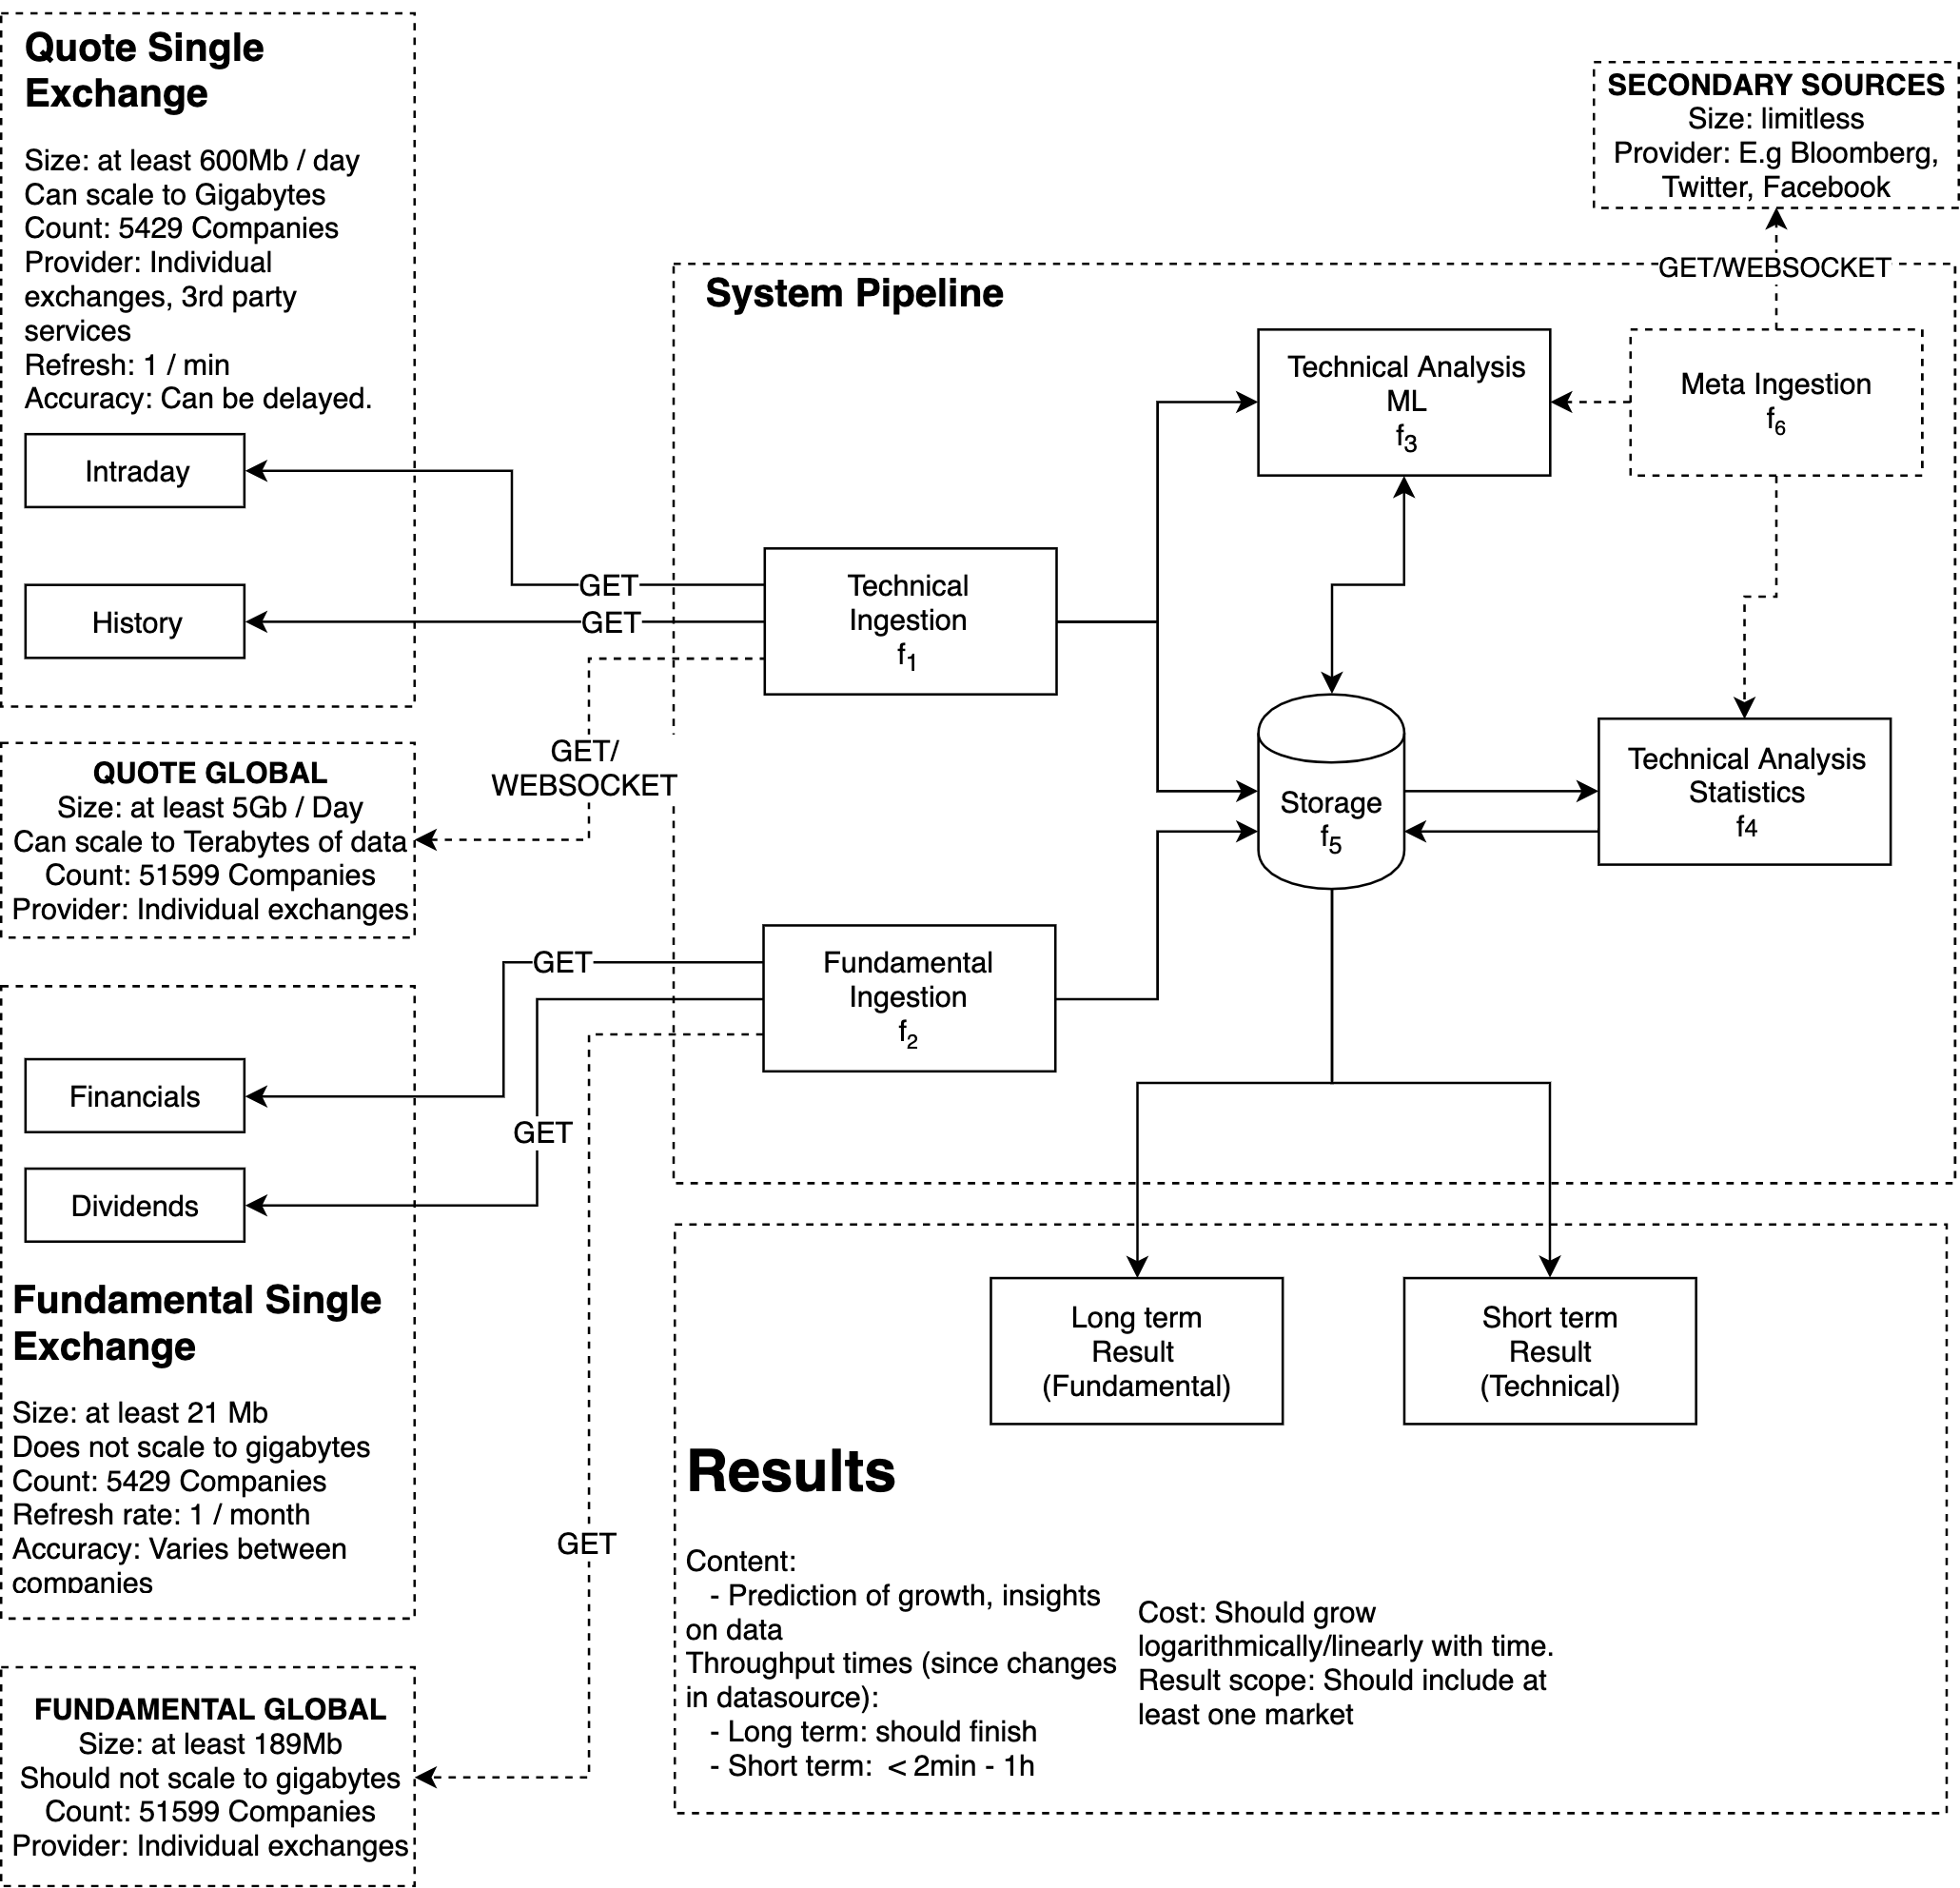
\includegraphics[scale=0.36]{images/system2} 
    \centering
    \caption{Example of a stock data pipeline}
\end{figure}

\section{Application scenario}
% research and engineering questions (why do you have to do it and why it is new)

To have a better picture what are the challenges of developing a system for technical analysis are, we will next look at a example case.
This is to give reader more practical and meaningful view on the problem at hand.

Somewhat normal system for analysing both fundamental and technical analysis is presented in figure 1.
In the figure, the components marked with solid lines represent the core system functions, and the dashed lines represent add-on functionalities that should be possible to extend into the system in the future.
The requirements of the system should be as follows;
The system should produce long ($r_1$) and short ($r_2$) term predictions of stock prices.
The computation of long term predictions can take time because of the nature of these predictions but the short term predictions should be between two minutes to one hour available.
Long term predictions are the result of fundamental analysis ($f_2$) and historical technical analysis ($f_4$) whereas the short term prediction should come mostly from quick technical analysis ($f_3$).
The cost of the system should grow logarithmically/linear with time meaning that the cost of processing and storing data should not exponentially increase over time.
Finally, the core system should be able to fulfill these requirements for at least the +5000 companies in the major U.S stock markets.

The data to the application is ingested from two main types of data sources quote and fundamental.
These sources consist of values that were briefly described previously in technical and fundamental analysis respectively.
The quote data is usually updated with minute intervals depending on the provider whereas the fundamental data does not change so often.
Theoretically, the fundamental data can change anytime, because of dividends which can be payed whenever the companies want but this does not happen often and these values are mostly used in the long term fundamental analysis so longer update intervals are acceptable.
In the figure, these are separated into the U.S market ones ($d_1$ and $d_2$) and the other sources ($d_3$ and $d_4$) that provide the same data on other global markets.
The extendable global data sources are grouped into one box but in reality this data would be ingested from numberable different providers as there is no single entity at the time of writing this that provides all of this data.
Theoretically the maximum size of this extendable data would be 5Gb per day which is extrapolated in from the U.S market data based on statistics that in January 2019 there were globally 51 599 companies listed in the stock markets \cite{global}.
This amount can and will fluctuate as companies enter and exit the markets but it gives us the scale of data we are working with.

Today, stock market analysis has also a large focus on predicting stock prices using secondary data sources that can have reflect and affect the prices of stocks. 
These secondary data sources can be anything but at the moment one of the most researched sources are traditional media and social media data.
Examples of using this kind of data to predict predict stocks can be found in \cite{kao}, \cite{skuza} and \cite{wai}.
This is why the system should have the ability to extend to ingest data from arbitrary secondary sources ($f_6$ and $d_5$ in the figure) to provide more versatile predictions about the stocks.
The amount of this data can be unlimited but is restricted to relevant sources.

Data is ingested from these data sources mainly using HTTP-protocol as this is the main method that these services ($d_1$ - $d_4$) provide.
Other possible methods that are usually available are Excel sheets and sometimes websockets, of which the websockets can be actually useful in cloud system, but as the HTTP-methods are currently the most used technology, this thesis is also going to focus on these.
Here we have separated the main ingestion functions into two main types of functions $f_1$ and $f_2$. 
$f_1$ is constantly polling and processing data whereas $f_2$ handles batch processing.
Both of these function store their raw output into the storage, but $f_1$ passes this also to the immediate technical analysis.

The system has two technical analysis functions.
For methdos that allow streaming updates there is $f_3$, which can for example be cumulative/reinforced ML models and for methods that need historical data in order to calculate the prediction, there is $f_4$.
For fundamental analysis, there is no a specific function as the introduced data sources usually provide these values pre-calculated and these values are usually easy to calculate dynamically with little to none amount of processing.

Finally, at the center of the system is the storage which is used to store the calculated predictions as well as the raw data from the data sources for later analysis.
For historical technical analysis, $f_4$, the storage should provide reasonable range query times when quering historical data and for the results the storage should provide efficient point queries for the results ($<$ 1s).

\section{Research Questions}

The focus of this thesis is going to be the part of the pipeline that calculates predictions based on historical data.
This means the ingestion, storage and analysis of this data.
As we have seen in the previous section, the system has to have the ability to grow, and we are going to focus on how to implement this in practice.

As the field of possible technologies is large, the main focus of this thesis would be the comparison of current relevant technologies in the context of stock data to help data scientists to decide what technologies to possibly use in their own projects.
The main result of this thesis would be information and possible tools that developers could use to develop this kind of system more efficiently.
Developers here can be people from companies that either do stock analysis as their main business or just want to analyze stock data efficiently.
These results could also be used in research to implement analyzing pipelines more efficiently so that the research group can focus on the analyzing of the stock data instead of worrying with getting the data to these parts.

Analyzing the stock data is also what most of the research today is focused on as this is the part that can actually produce profit.
This means that most papers ignore the steps of ingesting and storing this data.
Examples of this kind of papers are \cite{wu}, \cite{aghakhani} and \cite{kao}.
So one of the goals of this thesis would be to bring more comprehensive picture on stock data pipelines. 

This thesis will approach this subject from three different perpectives that cumulate on one another.
These perspectives are represented by the following three research questions:

What are the needs and requirements of this kind of system data-wise?
What are the methods currently used to conduct technical analysis and possibly what kind of data they use.
This thesis plans to provide the information on these so that when a reader is developing their own system they have a point of reference which they can use to evaluate their data sources.

What are technological options to implement a modern scalable timeseries analysis pipeline?
As there are enormous amount of different technological frameworks, this thesis plans to provide the reader information on the most promising ones currently.
This way the reader does not need to go through and learn variety of technologies in order to build their system.

How to implement big data framework for technical analysis in practice?
Finally the thesis plans to provide comparison and prototype implementations of stock data ingestion using the technologies that seem most prominent.
The metrics used to compare these systems would be the response time, possible scalability and the time it takes to develop these systems.
This is to save possible time of a person developing these when the trial and error is done beforehand and if the prototype system fits the developed architecture it can also be used as a basis for further development by the reader.

\section{Expected Outcome}

For the first research question "What are the needs and requirements of this kind of system data-wise?" this thesis plans to provide an analysis of the necessary stock market data and its usages.
From this analysis, the thesis would derive the main requirements for the system to fulfill in order to satisfy the needs of the possible subsequent analysis stage.
This result could then be used in the future if one would want to build their own ingestion system from the ground up as a base.

For the second question "What are technological options to implement this in practice?" the thesis would perform an analysis on the current trends in data ingestion solutions.
The thesis would provide information on the latest open-source technologies that could be used to implement this kind of system, how these would fulfill the requirements introduced by the first research question with application scenario and conclude this with a comparison of these technologies on what are the advantages of using one over another.
The result of this part could be used to decide what seems to be the most suitable technology to use to implement the application scenario technically. 

For the last question "How do the most viable big data ingestion options compare to one another in the context of stock data perfomance-wise?" the thesis would implement open-source prototype solutions based on the results of the second research question.
This prototype could be used by anybody (company or individual) as it is or as a base to build a more complex system on top of it.
The system would be targeted to practically implement the described application scenario, which could be used by companies with similar products allowing them to write more complex analysis algorithms based on the larger amount of data.

\section{Structure of the Thesis}

In the first chapter of the thesis we will be focusing on solving the first research question "What are the needs and requirements of this kind of system data-wise?".
The thesis would start by going through scientific papers about stock markets and stock analysis.
There would be first text generally about the characterics of the stock markets, what are they based on, what affects them, can they actually be predicted (random walk hypothesis) and so on.
Then the thesis would go through the main directions of analysing the stock markets (fundamental analysis, technical analysis) and explain briefly some of the methods (about three methods per direction) that characterize these directions (Gordon model, Magic formula, LSTM etc.) focusing on the data that these methods need in order to calculate their predictions.
This part would be concluded by deriving the requirements for the system based partly on these analysis methods and their data needs, and partly on the definitions that make up a scalable, secure and stable cloud system.
The next step would be solving the second research questions "What are technological options to implement this in practice?".
This step would perform literary research on what is currently used to perform big-data ingestion and storing, selecting from the list of technologies mostly those that seem to fulfill the requirements derived in the step 1 and would fit in the application scenario introduced in figure 1, specifically in $f_1$ and $f_2$.
For data ingestion, these technologies would probably be Apache NIFI, Apache Flume, Fluentd etc. 
For data storage, these could be HDFS, HDFS, Apache HBase, Apache Cassandra etc.
This step would consist of first introducing all of the selected technologies and going through how do they work, what are they supposed to solve and what are the advantages and disadvantages of using one.
After this, the section would do a comparison of these technologies in the context of stock data and conclude with analysis on which of the technologies would be the most prominent ones to solve this problem.
After this would start the experimental part of the thesis and the rest of thesis would be focusing on solving the final research question "How do the most viable big data ingestion options compare to one another in the context of stock data perfomance-wise?".
Based on the results of the step 2, I would implement couple of the most prominent solutions as a prototype systems.
This step would include the actual implementations and reporting of these implementations.
The report would consist of technical details; what parts does each of the system consists of, what versions were used, where the system was run etc. And subjective remarks; was it easy to implement, was there parts that did not fit together etc. 
The reporting part would also explain the metrics that would be measured for the subsequent analysis.
For these metrics, the dataset used to test the system would be the open-source REST API from IEX \cite{iex}, which is open for consumers until first of June, 2019.
These metrics could be, for example, the time it takes to batch process, processor usage, memory usage, database fetching times etc. 
As these systems would be run inside Docker containers, the tools used to measure these metrics would most probably be programming language specific functions and Docker specific statistics tools. 
In the final step, the thesis would first inspect the results from the step 3 and based on these make remarks on what could be the best potentially the best implementation in this context.
After this there would be an wrap-up on each of the previous sections concluding in retrospective what could've been possibly done better and what could be done in the future, concluding in recommendation what could be based on this thesis the best technical solution to implement system described in the application scenario. 


\chapter{Background}
\label{chapter:background} 

In this first chapter, we are going to look at the current stock market data analysis in big data environments.
This chapter is divided into two distinctive parts.
In the first part we will examine the current state of stock market data analysis in big data environment.
This includes the methods and pipelines used to conduct this in real life.
In the second part we will use the result of the this first section and study the most promising big data technologies that could be used to implement pipelines that analyze the stock data.

% Guiding instructions from the thesis example
%The problem must have some background, otherwise it is not
%interesting.  You can explain the background here. Probably you should
%change the title to something that describes more the content of this
%chapter. Background consists of information that help other masters of
%the same degree program to understand the rest of the thesis. Often
%the background has two parts: the first part tells the theoretical background
%and the second one describes the background tied to the implementation.

%Transitions mentioned in Section~\ref{section:structure} are used also
%in the chapters and sections. For example, next in this chapter we
%tell how to use English language, how to find and refer to sources,
%and enlight different ways to include graphics in the thesis.

\section{Stock market analysis}

In order to build practical stock analysis systems, we start by looking at the methods of stock data analysis to understand the underlying domain.
Stock market analysis is an enormous domain by itself and there are multiple ways to approach this data.
For example possible problems to solve are finding anomalies in the data, predicting the future price and analysing the possible causalities.
In this thesis we will be approaching this from the price prediction perspective which can also be used as a tool in other problems such as anomaly detection \cite{islam}.

In this chapter we examine what are the state-of-the-art methods that researchers use to analyse stock market data.
We are especially focusing on methods that in some way use big data for this analysis.
We will be also inspecting real-life implementations of stock data analysis and examine some of the existing big data pipelines for stock market analysis focusing on what are the technologies used to build these.

\subsection{Stock price prediction}

The current methods on stock price prediction can be divided roughly into two different categories; statistical methods and machine learning methods.
Both of these categories can be further divided into fundamental and technical analysis categories depending on what data they use as a source of analysis, but these categories overlap a little because of new ensembled models.
With statistical methods we mean here the traditional mathematical models that need quite a lot of understanding of the domain in order to derive them.
With machine learning methods, we mean algorithms and statistical models that derive underlying principles from data using patterns and inference.

Both of these methods are trying to beat the efficient market hypothesis (EMH).
EMH states that the all the current public information available should already be seen in the price of the stock.
In other words, the only thing that can affect the price of the stock would be unknown new information and the randomness of the system, which leads to a claim that stock prices can not be predicted using historical data.
However, there have been multiple studies shown that this hypothesis could possibly be beaten using big data. \cite{nam}
This hypothesis has also been challenged with overreaction hypothesis that states that the market overreacts to new information making it possible to somewhat predict the market before the prices change \cite{day}.

\subsubsection{Statistical methods}

The driving force of stock analysis in the past have been the statistical methods and there are still a lot of new papers analysing stocks using these methods.
There are countless to approach this problem from statistician point of view so here we have listed only some of those that have some relevance to the subject of this thesis.

From the technical analysis perpective, where only the data related to the price of a stock is analysed, we will be looking at momentum indicators. \cite{utthammajai}
Momentum indicators, as the implies, measure the speed of change in the stock prices and investors make decisions based on the thresholds of these values whetever a stock is being overbought or oversold. \cite{james}
When searching research on big data usage in technical analysis there are some key indicators that show up frequently.
These are relative strength index (RSI), moving average convergence divergence MACD and Williams \%R which are all momentum indicators.
These indicators can be used as they are but these have been also used as features that machine learning algorithms use to predics prices. \cite{serez}

All of these indicators measure the momentum of the price, but they all do it differently.
RSI and Williams \%R are both called oscillators because their values oscillate between maximum and minimum values they can get.
Where as MACD compares long-term and short-term trends to predict if there is currently a notable trend.
Because of the differences in the formulas and the factors that these values are measuring, the results from these formulas can be conflicting which can help to recognize one indicators bias when using multiple different indicators. \cite{james}

Moving away from the momentum indicators, Autoregressive integrated moving average (ARIMA) models have also been successful way of analysing time series stock data and they have been also used with big data. \cite{wang}
However, with the new advances in machine learning, there seems to better performance to be achieved with machine learning methods. \cite{khashei}
Due to this and the complexity of ARIMA models, we will only briefly make a note of them here and focus more on the machine learning methods in the next section.

In the fundamental analysis side, most of the recent developments have happened with textual data from news and social media using machine learning methods meaning that traditional statistical methods have not gained that much interest recently.
However, as there is a lot of relevant financial big data that can be used with traditional methods, here are couple of recent examples of the usage of this kind data:
Day et al. \cite{day} tried to link oil prices to stock prices using global financial data streams with stochastic oscillator techniques.
Kyo \cite{kyo} combined technical and fundamental analysis by using regressive model that takes into account business cycles in Japan's stock market.

\subsubsection{Machine learning methods}

As stated before, machine learning is the current trending stock analysis methology that has gained a lot of interest.
Both supervised and unsupervised learning techniques has been tried to predict the prices but recently neural networks especially have gained a lot of interest due to their adaptablity to any non-linear data.
Neural networks have the advantage that they usually do not need any prior knowledge about the problem and this is the case when we are looking at seemingly random stock market data.

We start by looking at neural networks used to predict the market using only the market data (technical analysis data).
There are multiple different neural network architectures to choose from and the most popular one currently seems to be a basic multilayered feed forward network (MFF) when analysing only the stock market data.
There is some results that have shown that increasing the size of MFF, by adding layers and neurons, can produce better results.
This however, increases the amount of needed computation and will probably have some upper bound before it starts to overfit the training data. \cite{senguptaa}

Although MFF is seemingly the most popular, better results have been able to achieve with convolutional neural networks (CNN) and long short-term memory (LSTM).
With convolutional neural networks, the upper hand to regular MFF seems to be the ability to express same amount of complexity with smaller amount neurons, although no direct comparisons have been made with these two.
With LSTM however, it has been directly shown that it performs better than other memory-free machine learning methods including MFF.
As stock data is literally a time series, the LSTM's ability to remember previous states seems to separate it with other methods.
There currently seems to be no papers on how the LSTM performs compared to CNN so we can only assume that the performance of these two is pretty close when it comes to the complexity of the network.
After these standalone architectures the next step to seem to be hybrid architectures combining more than one model into one and this has already achieved seemingly better results than these standalone models. \cite{senguptaa}

In order to train a neural network to predict stock markets we need features and classes to label these features correctly.
Because there is such a huge amount of data in stock transactions, manual labeling is not an option.
The simplest way automatically generate features is to take calculate change in price in each time step.
This way the network can for example output simple binary classification telling whetever the price is changing more or less than median price. \cite{fischer}
When we take this to a bit more complex level, similar features can be made from RSI, MACD and Williams \%R values which we introduced in the previous section. \cite{serez}

When we move on to the fundamental analysis, similar kind of networks are used to with financial news and social media data.
Again LSTM and ensemble models are used to connect this data from outside with the price trend of stock market.
There are research using just general social media data that concerns the whole market but there are also usages of stock specific posts.
Fundamental data that is in textual form, term frequency–inverse document frequency (TF-IDF) is a common choice to present features \cite{chungho}.
This data is then classified based on the general sentiment that they seem to represent.
Positive sentiment toward company would lead to the rise of stock price and negative sentiment vice versa.

\subsection{Existing pipelines}

We then move on to examine the actual implemetations that do this analysis.
For this section, we examined 19 different stock data analysis pipeline that handle or are able to handle big data.
The big data might not be the actual stock data but for example social media data that was used to analyse the actual stock data.
Information about these pipelines were all publicly available, although most of the pipelines were not open-sourced.
Fourteen of these pipelines were reported in academic publications and the rest five are, or at least have been, in industrial use.
There were also multiple open-source pipelines that have been developed for big data stock analysis, but information about the actual usage of these pipelines were not found.
This is why we excluded these from this study in order to get more relevant results.

We have divided this section into subsections based on different parts from the pipeline starting from the furthest away of the possible clients and moving our way up towards the analysis phase.
The biggest problem here is that the companies that work in the forefront of stock analysis, seldom share their software achitectures for business reasons.
Nevertheless, with the public information available we can get an excellent view of the state-of-the-art pipelines in academic world and a general idea how the pipelines are build in the industry side.

It is also not that easy to compare technologies used in academia and industry.
Both have different needs and goals that they wish to achieve.
In academia, the pipeline is usually made in ad-hoc manner trying to minimize the time used for development and maximise the time needed for testing.
This is possible, because researchers do not have same client side restrictions that industry might have.
In industry side, it is usually important that the pipeline stays operational during the whole livecycle of the system.
Where researchers only need these pipelines in order to conduct a couple of experiments, these industry pipelines have to survive possibly multiple of years of usage.
These industry pipelines also serve the results to multiple clients that all expect small latencies from the system in order to use the system efficiently whereas in academia, this is not a requirement but helps the research to be made efficiently.
So bearing these domain-specific requirements in mind, different technologies can be used to achieve optimal solution in different situations.

\subsubsection{Data sources}

Stock market data is not cheap.
This is mostly because the exchanges that run the stock markets, usually make most of their profit with trade data and thus do not want to give this data freely away.
There are however services who do provide part of this data with a much lower cost available to companies and researches which cannot possibly afford the complete real-time data.
This partial data usually consist of historical end of day data, which is the aggregated statisctics of the stocks after the market has closed for the day.
Although this data is complete in the sense that it tells all the necessary information about stocks price evolution on a day level, we will be referring this data as the aggregated data during this thesis and reserve the term complete stock market data for the data that contains all of the transactions.
What this means for the systems is that the stock data can exponentially smaller at the beginning of pipelines lifecycle when there possibly is no way to access the complete stock market data, but system must be able to scale to this complete data set size when time progresses.

In academic papers, the Yahoo Finance API has been the de facto service used as the source of this partial stock data. \cite{islam} \cite{adresic} \cite{le} \cite{serez}
Unfortunately, although this service have been used in papers published in 2019, this API was shutdown by Yahoo in 2017.
Today, there are no service that provides the same amount of data that this API did, but some substituting services do exist.\cite{lotter}
These services will be introduced more completely in chapter 4 where we will evaluate which one to use in the implementation chapter.

\subsubsection{Used technologies}

We then move on to examine the actual technologies and frameworks that are in use by starting from the furthest away from the client, the ingestion layer.
With ingestion we mean the part of the pipeline that handles fetching and initial processing of the data.
This step with stock market data varies a lot depending who is fetching the data and for what purpose.
The most common method for ingesting stock market data was found to be custom scripts.
This is because the format of ingested data can vary greatly and scripts are relatively easy to write.
This is usually enough with the aggregated stock market data, however, it does not scale.

Common big data technologies are usually introduced when the system has to ingest for example great amounts of textual data such as news and social media feeds.
For these purposes, the most common technology in scientific papers is Apache Flume which is used, for example, in \cite{peng} and \cite{das}.
Another framework that is commonly reported in the ingestion step is the Apache Kafka streaming platform. \cite{chungho} \cite{juan}
Both of these are open-source frameworks which makes their usage relatively cost-free.
In the industry side the usage of ready-made services from cloud providers are common.
These services are for example the Google Dataflow as in \cite{palmer}.

After the ingestion, the data has to be stored.
Stock market data is quite structured by itself but the data from third-party sources used to enrich stock data is usually not.
This puts a restriction on what are the possible storage options available.
Academic papers usually do not have to worry about this as the systems just have support ad hoc calculations but in the company context this becomes a crucial part of the system as it is the component that enables low latency responses without having to fetch data all the way from the original data source.

With big data systems there is usually two options which are either cloud platform specific products or open-source HDFS-based systems.
This is also the case with stock analysis systems.
From the cloud platform products, there are information on usage of Amazons S3 and Googles BigTable with BigQuery. \cite{snively} \cite{palmer}
In the open-source side HBase \cite{gu} and Cassandra seem to be the two most openly used database solutions.

Then as we finally have the data in control, we can apply some analysis to it.
In the analysis phase, there is not that much variety in used technologies.
Apache Spark with its MLlib library is dominating this field with its capabilities to process data efficiently. \cite{islam} \cite{chen} \cite{chungho} \cite{adresic}
Where Apache Hive and Apache Pig were previously most used technologies, now Spark seems to be taking their place \cite{snively}.

In the industry side, there is indications of Apache Storm being used with real-time classification \cite{juan}.
The strong point of Spark is that same models can be used with Spark Streaming framework, but better latencies can be achieved with Storm making it possibly better choice for companies which have resources to implement two separate systems \cite{kumar}.

\subsubsection{Monitoring}

Finally we are going to examine one specific charasteristic which is usually ignored when pipelines are reported.
Good monitoring is essential to ensure that the pipeline is running correctly and optimally.
In the next few paragraphs we explain a bit more about the importance of monitoring as this is one of the areas that we will focus while trying to create a stock data pipeline.

None of the public sources on pipelines that were examined for this chapter reported exatly how they monitored their pipelines in practice.
In cases where for example Spark is used, we can assume that the process is monitored using Sparks own monitoring tools which measure load and resource usages.
These tools are valuable to measure the perfomance of the application, but they do not always tell the whole truth about the applications state.

With pipelines that analyze massive amounts of data, the quality of data is very important.
This is not only when choosing what data source to use but the data must be kept from corrupting during the whole pipeline and to ensure this good monitoring is essential.
Perfomance monitoring can pick up these corruptions if the corruption is large enough to make the program crash.
However, in most cases this corruption can be only a change in values that would pass as an input.
This would then lead to erronous results which could take quite a bit of resources to calculate.

So in order to make right decisions concerning models and save time while training, it is crucial to identify these kinds of problems early as possible and this is why we need good monitoring.
In the next chapter, we will be looking more closely on the technologies that could be used to build a pipeline that can conduct modern stock analysis.
We will also examine couple of different ways to monitor the system in order to prevent problems that were raised in this section.



\section{Big Data Technologies}

In this section, we will examine more carefully the technologies that can be used to implement a stock data pipelines in the big data context and try to answer the second research question in the process.
We have gathered here technologies that we saw used in existing big data stock pipelines in the previous section.
We also added couple of promising frameworks that could be used in the pipelines but there is no public information about companies using them yet.
To keep this section compact and more useful for majority of the novice data scientists that do not possibly have access to costly resources, we have included only the open-source solutions here leaving outside the services that cloud providers offer such as Amazon S3 for storage or Google Dataflow for ingestion.

\subsection{Data ingestion}

Here we will be using the same definition for ingestion as before; data fetching and initial processing which includes data validation.
This is one of the crucial parts of the pipeline as it is responsible of turning arbitrary data into facts that the rest of the pipeline can use and rely on.
This also makes it the hardest part to develop as the developer must understand the data well enough that these parts can work efficiently and prevent erroneous states in the later stages of the pipeline.

We have gathered here three main technologies that are usually mentioned when developers are talking about open-source data ingestion, but in reality all of these frameworks have a bit different tasks they try to fulfill.
This makes comparing these technologies harder and it usually just means that the better technology here is usually the one that is better suited for the current problem, which does not make the other ones any worse than the selected one.
On top of Apache Flume and Apache Kafka which were already used in existing pipelines, we have also included here Apache NiFi which has promising features that could be suitable for our use case.

\subsubsection{Apache Flume}

Apache Flume is one of the Apache Software Foundation (ASF) projects that is quite popular in the context of ingestion.
From the projects official website we have definition that Flume is "distributed, reliable, and available service for efficiently collecting, aggregating, and moving large amounts of log data" \cite{flume}.
So the main focus of Flume is to manage log data, but as we have already seen, this is not the only use case for this tool.

Flume was first introduced by Cloudera in 2011.
In same year, it was officially moved under ASF and came out of the incubation phase the following year.
During this incubation, developers had already started to refactor the Flume and the result of this is the 1.X lineage of Flume which is still going to this day. \cite{hoffman}
At the time of writing this the latest production-ready version is 1.9.0.

Flume's high level architecture can be divided into 3 different parts: sources, channels and sinks which all run inside an agent which is an abstraction for one Flume process.
Data is inputted to the system from the sources, then it goes through channels and is finally written into sinks. 
While going through channels the data can be processed using functions that Flume calls Interceptors. \cite{hoffman}

The main unit used of data in Flume is called Event which is structured like most of the other message formats you can find in network protocols.
Event has a header, which is key-value pairs of meta data and a body which usually is the actual data. 
Overall, Flume architecture is message driven which allows it efficiently to multiplex data across multiple computing instances leviating the work load between these machines. \cite{hoffman}

When processing large amounts of data, it is important to avoid bottlenecks that can form in the pipeline and this is why knowing the amount of data flowing through Flume is extremely important.
Bottlenecks that can form in Flume are for example cases where data is coming from sources faster than the Flume is able to write to sinks.
These kind of situations can be avoided with the knowledge of the data domain when configuring Flume instances but also by monitoring Flume processes in order to respond to these kind of situations. \cite{hoffman}

\subsubsection{Apache Kafka}

Apache Kafka describes itself to be a "distributed publish-subscribe messaging system" and it can be used for three different purposes: as a messaging system, as a storage system and as a stream processor. \cite{kafka}
Because we are examining Kafka in the context of data ingestion, we are mostly interested in its messaging and stream processing capabilities, but it's good to keep in mind that it is possible to store data with Kafka for a longer time if necessary.

Before being a ASF project, it was first developed by LinkedIn to gather user activity data in 2010. \cite{ramalingeswara}
After being released from incubation in 2012 many other big industrial companies such as eBay and Uber \cite{yuan} have taken kafka into use to manage their own enormous data systems.
Today, Kafka is already in its version 2 and can be integrated with almost any modern big data framework. \cite{ramalingeswara}

Kafka operates on publish-subscribe architecture where producers input data into the system by producing data and consumers subscribe to the data which they want to consume/receive.
To make this work with big data, Kafka has a core abstraction called topic which has multiple immutable queues called partitions.
When producers produce new data, this data is appended to a partition queue where where Kafka keeps track which items consumers have already consumed by tracking the offset of a consumer in a queue.
With this kind of architecture Kafka makes promises that the data retains its order throughout the system and does not arrive to consumers out of order.

As for the scalability of this kind of system, a single partition must fit onto a single server, but topic which has multiple partitions does not have this limitation and this allows topics to scale over the Kafka cluster.
Fault-tolerancy can be achieved by just replicating these partitions over the cluster.
Multiple consumers can form consumer groups that consume some topic simultaneously from multiple partitions meaning that in addition of Kafka being itself scalable cluster, it allows its consumers to be also scalable cluster and without any additional complexity. \cite{kafka}

\subsubsection{Apache NiFi}

Apache NiFi was made to dataflow management and its design is inspired by flow-based programming.
It was originally developed by National Security Agency (NSA) as a system called "Niagara Files" and was moved under ASF in 2014 making it the newest addition under ASF out of these three intoduced ingestion technologies. \cite{bridgwater}

As we have seen already with the last two ingestion frameworks, all these frameworks have their own abstractions for data and the processes that handle this data.
NiFi's core abstraction is FlowFile which represents the data that flows through the system. 
These are processed with FlowFile Processors that are connected to each other by Connections and these can be grouped into Process Groups.
These processors and their connections are then managed by a Flow Controller which acts as the brain of each node in a NiFi cluster. \cite{nifi}

NiFi cluster follows zero-master clustering paradigm meaning that the cluster does not have clear master nodes and vice versa no slave nodes.
Every node in NiFi cluster processes data the same way and the data is divided and distributed to as many nodes as needed.
Apache ZooKeeper is used to handle failure of nodes in the cluster.\cite{nifi}

\subsection{Data storage}

Data storage forms the center of the pipeline and is one of the major places where bottlenecks can form.
Possible bottlenecks are the query latency and the writing speed which can slow the whole application down if not implemented efficiently enough.
If this non-trivial task was not enough, the data storage must also be able to resist error states that could occur when the hardware malfunctions for example with power outages or network outages.
We have gathered three major big data storing technologies that were used in existing pipelines: HDFS, HBase and Cassandra.
We start with the HDFS and move towards more industrially used systems.

\subsubsection{Hadoop distributed file system}

Hadoop distributed file system (HDFS), which is the core part of Apache Hadoop ecosystem, is one of the current defacto ways to store big data.
It has gained a lot of popularity with the map-reduce programming paradigm.
HDFS build so that it does not have to be run on high quality hardware, normal commodity hardware is more than enough to run the system.\cite{hdfs}

HDFS offers all the same functionalities that a traditional file system would offer.
Clients can create, edit and delete files which can be stored into directories that form hierarchies.
What makes HDFS differ from a normal file system is its ability to handle a lot larger data sets and at the same time have a better fault-tolerance than a traditional file system.\cite{hdfs}

HDFS is based on a master-slave architecture where the master is called NameNode and slaves are called DataNode.
The NameNode stores and manages the state of the whole system and the actual client data never flows through this node.
The data is stored into the DataNodes which manage this data based on the instructions that the NameNode gives them.\cite{hdfs}

For reliability, data is replicated between DataNodes so that the outage of individual DataNodes does not affect the overall perfomance of the system.
In order to identify and react to these kind of failures, each DataNode send heartbeat-like messages to the NameNode, which then conducts needed actions if a heartbeat is missing.
The NameNode itself, on the other hand, is a single point of failure.
It does record the changes and the state of the system into files called EditLog and FsImage which can be used to replay the changes in the system if NameNode goes down temporarily and because of these files are crucial to get the system back up, usually multiple copies of these are stored into disk. \cite{hdfs}

\subsubsection{Apache HBase}

HDFS by itself is only made to store very large files, so the methods it provides our quite limited.
This is where the Apache HBase comes in which is implemented based on Google's BigTable framework.
Where BigTable uses Google's own file system, GFS, HBase is build on top of HDFS. 
HBase is a NoSQL database altough it does not natively have many features that a normal database would have.
Notably, it does not have its own advanced query language.\cite{george}

HBase's record structure is somewhat similar to its relational counterparts.
Data is stored into rows that consist of columns, that are identified by a unique row key.
Rows form tables and tables can be further grouped into namespaces.
The difference to typical relational data model comes after this.
Columns may have multiple versions and timestamp information about the column and its version are stored into separate entity called cell.
The columns do not form table like structures with rows, and instead act like key-value pairs which can be grouped into column families.
This way values that would be for example 'null' in normal relational database, do not take any room in HBase as such key-value pairs can be omitted. \cite{george}

HBase's core abstraction of scalability is called Region.
Region is a set of continous rows that are split when one Region grows too large.
Each region is served by a single RegionServer and each RegionServer can serve multiple Regions.
So Hbase cluster is scaled by adding these RegionServers which can serve more Regions to clients. \cite{george}

HBase does not instantly store changes into disk. 
Changes are first recorded into a log called write-ahead log (WAL) and after this the change is stored into a memstore which is in memory.
After the changes expire in the memory, the changes in memory are flushed into the disk as they are, into a file called HFile. 
In order to avoid large amounts of small HFiles in the disk, HBase periodically merges these files using a process called compaction.
These are done in file scale (minor compaction), but also in larger scale where all the files inside one region are merged into one and data market for deletion can be cleaned in the process (major compaction). \cite{george}

\subsubsection{Apache Cassandra}

Apache Cassandra is a NoSQL database that is build on peer to peer architecture.
Cassandra provides its users same tools that a normal relational database would.
Its record structure is the same with rows, columns and tables such as with typical relational database and it provides a SQL-like query language.
What differs Cassandra from a normal relational database is its scalable architecture which we will be looking next. \cite{yarabarla}

Cassandra's main scalable units are called Nodes that are a single instance of Cassandra running in a single machine.
These Nodes are grouped together based on the data they serve and these form Rings.
Data distributed and replicated between the nodes based on the hash of data's partition key.
With consistent hashing algorithm, every Node has the same amount of data. \cite{neeraj}

Unlike HBase, Cassandra does not guarantee the consistency of data due to CAP theorem but instead guarantees the availability at all times.
Cassandra implements "tunably consistent" paradigm where user can define for each write/read to be consistent with the cost of availability.
This high availability, makes Cassandra better choise for example web application where the data must be available at all times, but the data doesn't necessary have to be up to date. \cite{neeraj}

\subsection{Machine learning frameworks}

When we researched existing pipelines we noticed that machine learning libraries such as Tensorflow and PyTorch are still quite used even when data can scale to enormous amounts.
This is partly due to their support for processing data with GPU.
This allows them to perform really well in single machine instances while needing minimal time to develop.
But when these are run with data which size is scaled to terabytes, development becomes a bit more harder as this is not the environment these are designed to run at.

As we saw in the previous chapter, the Apache Spark framework with its Spark ML library is currently the most used big data machine learning platform.
Spark, however, natively supports only classical machine learning models and currently has no native deep learning solutions, which are the state-of-the-art methods we are interested in.
Spark is still a highly efficient processing framework for big data and the de facto technology in the market with its good integrations with the frameworks we already introduced and its mature ecosystem.
That is why we are next going to briefly look at how the Spark ecosystem works and then move on to see tools which we can use to train deep learning models in Spark ecosystem without writing implementations from scratch.

\subsubsection{Apache Spark}

Apache Spark is a distributed in-memory data processing system that provides tools for scalable data processing.
Spark has a master-slave architecture, where a driver node acts as a master and executes Spark program through Spark Context.
The driver node passes tasks to worker nodes that the Spark Context together with Cluster Manager manages.
The most popular cluster manager currently seems to be YARN but Mesos or Spark's own standalone could also be used for this job. 
Each worker node then has its own executor process which runs the given tasks in multiple threads when necessary.\cite{spark}

Until version 2.0, Spark's main programming interface was a data structure called Resilient Distributed Dataset (RDD).
RDD is a collection of elements that can be partiotioned throughout the cluster allowing them to be processed in parallel accross multiple servers.
RDD's are still in use for backward compatibility reasons, but from version 2.0 onward Spark's main abstraction has become structure called DataSet.
DataSet is similar to RDD in high level, but it provides richer optimizations under the hood and higher level methods to transform the data.
With the DataSets, a new abstraction called DataFrame was introduced which is can be compared to a table in relational database.
DataFrame is a DataSet of Rows that can be manipulated with similar methods that you could do for DataSet.\cite{spark}

Spark has divided its functionalities into sub-modules that are specified into specific tasks such as Spark Streaming for stream processing and SQL for processing data in tabular form.
We are mostly interested here in Spark ML module.
Spark also has a module called Spark MLlib which some of the research still use.
The main difference between Spark ML and MLlib is that Spark ML provides newer DataFrame API whereas MLlib uses older RDD datastructures.\cite{amirghodsi}

% There is some confusion because of this naming, but according to Spark's own documentation neither of these libraries have been deprecated and Spark ML is just DataFrame extension to MLlib library.
% However, Spark ML is said to be the primary API and no further features are going to be developed in the MLlib API.
% Spark ML is also referred to not be the real name of the DataFrame version, but it has stuck with community because of naming of the packages.
% For general convenience reasons, we are going keep referring the DataFrame version of the machine learning library as Spark ML, but reader should be aware of its relationship with the RDD based library.\cite{spark}

Spark ML provides whole set of classical machine learning algorithms such as linear regression, naive bayesian and random forests.
It also has a concept of pipelines which consist of different transformers and estimators, which are made to make model developing easier.
However, the main problem with Spark ML is that it does not have natively tools to implement deep learning models on Spark.

\subsubsection{Deeplearning4J}

Deeplearning4J (DL4J) is distributed framework of deep learning algorithms that work on top Spark and Hadoop ecosystems.
It provides all the most popular deep learning models such as multilayered networks, convolutional networks, recurrent networks.
DL4J also provides a lot of tools for preprocessing the data before fed for training in the form of sub-projects. \cite{dl4j}

In distributed environment DL4J trains its models using Stochastic Gradient Descent (SGD).
This is implemented in parallel on each node of the cluster using either of the two methods that the DL4J offers, gradient sharing or parameter averaging.
From these two, the first one has become the preferred way to implement SGD in DL4J starting from its latest release and this is why we are going to ignore the technicalities of the latter one for now.

In the gradient sharing approach, the gradient is calculated asynchronously on each node in the cluster.
The main idea behind DL4Js implementation of this, is that not every update on the gradient is sent to every other node.
Each node has a threshold which defines when a change is large enough to be shared with the global gradient.
This combined with its own heartbeat mechanism provides efficient and fault tolerant way of training a model in distributed environment. \cite{dl4j}

In academia, DL4J is not that used as its main language is Java, but this choice of language makes it really suitable for industrial use.
However, DL4J supports Keras model import which allows user to use other languages than the JVM based alternatives.
This makes python based prototype systems be able to run in industrial Spark cluster. \cite{dl4j}

\subsubsection{Apache SystemML}

Apache SystemML is a bit different machine learning system when compared to Spark ML and DL4J.
Similarly to DL4J, SystemML also runs top of Spark, but unlike DL4J it is not a straight forward programming library.
SystemML has its own R- and Python-like declarative machine learning languages (DML), which can be used to define machine learning algorithms that run on the Spark. \cite{systemml}

Currently, these languages cover about the same use-cases that Spark ML does.
What makes SystemML differ from Spark ML is that deep learning models developed in Keras or Caffe can be converted into DML.
So theoretically SystemML supports deep learning through these libaries although its core methods do not have these methods.
This allows it to be run on classical command-line interface, but also from jupyter notebooks which are currently vastly in use in academia. \cite{systemml}

\subsection{Monitoring}

We have already seen quite a bit of framework specific monitoring solutions, which cover monitoring individual components in the pipeline.
Next we will take this monitoring a step further and look at monitoring solutions that work outside of these components and can be used to monitor the global state of the pipeline.
This can make monitoring easier when all the information is available in one place and it also helps to infer cause-effect relations.

We have gathered here two different monitoring solutions for two different needs.
The ELK stack for monitoring the data flow inside the system and individual components and the ModelDB to specifically monitor the Machine learning models that are produced by the pipeline.

\subsubsection{Log monitoring}

The most common solution for monitoring logs in bigger system is the ELK stack. 
ELK stack which is an acronym for Elasticsearch, Logstash and Kibana stack, is a common stack used to implement collection of logs and their visualization in Big Data environment.
The need for such as elaborate stack for just collecting logs, comes from the fact that when you have a big data system, the logs of such a system form a big data problem of their own, so in order to solve this problem this stack was developed.
It provides scalable data ingestion system, with a distributed storage that can be accessed and visualized in efficient manner. \cite{elastic}

In this stack, Logtash, an open-source data ingestion pipeline tool, is used to ingest the log data.
This ingested data is the stored into Elasticsearch which is a distributed search and analytics engine, which provides REST interface.
Finally, the data stored into Elasticsearch can be visualized and monitored with Kibana, which is a tool developed to do just this. \cite{elastic}

Because of different user needs the stack has evolved into stack that the company behind these technologies calls Elastic Stack.
This stack really only differs from ELK-stack by a component called Beats, which can be used to build more lightweight stack for simpler needs.
However, pure ELK stack is still very popular option to handle log data. \cite{elastic}

\subsubsection{Machine learning monitoring}

Open-source monitoring tools that are specifically designed for machine learning are not that common, but couple of tools do exist.
These tools do not only help monitor the models perfomance, but also provide tools for deploying and versioning these models just like developer would use git to manage their code base.

ModelDB is a system developed in Massachusetts Institute of Technology (MIT) for ML model management.
It provides tools that can be used to monitor the performance of models and compare these results with each other.
It also allows logical versioning of models and helps to reproduce the models this way.
ModelDB, however, does not support models from many different ML libraries and currently the only supported libraries are Spark ML and scikit-learn.
The library is said to have second version coming up, but at the time of writing this the library has not had major update for an year.
\cite{modeldb}

Another, newer option is an open-source project called MLFlow.
It does all the same things that the ModelDB does, but markets itself as a more end-to-end solution.
On top of tools for the managing explained in ModelDB paragraph, MLFlow puts more emphasis on packaging the models and the deployment of these models into actual use.
\cite{mlflow}

Unlike ModelDB, MLFlow does not care about what is the library that generates models.
It does this by providing CLI and REST API's that can be integrated with the system ignoring the underlying technologies.
For convenience, it also provides APIs for Python, R and Java which can be used for tighter integration.
MLFlow is as project quite young having its first full version released in June 2019, but it has a healthy development community and is actively developed.
\cite{mlflow}

\chapter{Big Data Technologies}
\label{chapter:environment}

%A problem instance is rarely totally independent of its environment.
%Most often you need to describe the environment you work in, what
%limits there are and so on. This is a good place to do that. Sometimes
%the environment is described together with your own implemantation, in
%the same chapter. Here, we first tell you about the LaTeX working
%environments and then we have an example from an thesis written some years
%ago.

In this chapter, we will examine more carefully the technologies that can be used to implement a stock data pipelines in the big data context and try to answer the second research question.
We have gathered here technologies that we saw used in existing big data stock pipelines in the previous chapter.
We also added couple of promising frameworks that could be used in the pipelines but there is no public information about companies using them yet.
To keep this section compact and more useful for majority of the developers that do not possibly have access to company level resources, we have included only the open-source solutions here leaving outside the services that cloud providers offer such as Amazon S3 for storage or Google Dataflow for ingestion.

\section{Data ingestion}

Here we will be using the same definition for ingestion as before; data fetching and preprocessing which includes data validation and feature extraction.
This is one of the crucial parts of the pipeline as it is responsible of turning arbitrary data into facts that the rest of the pipeline can use and rely on.
This also makes it the hardest part to develop as the developer must understand the data well enough that these parts can work efficiently and prevent erroneous states in the later stages of the pipeline.

We have gathered here three main technologies that are usually mentioned when academics are talking about data ingestion, but in reality all of these frameworks have a bit different tasks they try to fulfill.
This makes comparing these technologies harder and it usually just means that the better technology here is usually the one that is better suited for the current problem, which does not make the other ones any worse than the selected one.
On top of Apache Flume and Apache Kafka which were already used in existing pipelines, we have also included here Apache NiFi which promising features that could also be used for this task in this kind of system.

\subsection{Apache Flume}

Apache Flume is one of the Apache Software Foundation (ASF) projects that we will be seeing a lot especially in the context of ingestion.
From the projects official website we have definition that Flume is "distributed, reliable, and available service for efficiently collecting, aggregating, and moving large amounts of log data" \cite{flume}.
So the main focus of Flume is to manage log data, but as we have already seen, this is not the only use case for this tool.

Flume was first introduced by Cloudera in 2011.
In same year, it was officially moved under ASF and came out of the incubation phase the following year.
During this incubation, developers had already started to refactor the Flume and the result of this is the 1.X lineage of Flume which is still going to this day. \cite{hoffman}
At the time of writing this the latest production-ready version is 1.9.0.

Flume's high level architecture can be divided into 3 different parts: sources, channels and sinks which all run inside an agent which is an abstraction for one Flume process.
Data is inputted to the system from the sources, then it goes through channels and is finally written into sinks. 
While going through channels the data can be processed using functions that Flume calls Interceptors. \cite{hoffman}

The main unit used of data in Flume is called Event which is structured like most of the other message formats you can find in network protocols.
Event has a header, which is key-value pairs of meta data and a body which usually is the actual data. 
Overall, Flume architecture is message driven which allows it efficiently to multiplex data across multiple computing instances leviating the work load between these machines. \cite{hoffman}

When processing large amounts of data, it is important to avoid bottlenecks that can form in the pipeline and this is why knowing the amount of data flowing through Flume is extremely important.
Bottlenecks that can form in Flume are for example cases where data is coming from sources faster than the Flume is able to write to sinks.
These kind of situations can be avoided with the knowledge of the data domain when configuring Flume instances but also by monitoring Flume processes in order to respond to these kind of situations. \cite{hoffman}

\subsection{Apache Kafka}

Apache Kafka describes itself to be a "distributed publish-subscribe messaging system" and it can be used for three different purposes: as a messaging system, as a storage system and as a stream processor. \cite{kafka}
Because we are examining Kafka in the context of data ingestion, we are mostly interested in its messaging and stream processing capabilities, but it's good to keep in mind that it is possible to store data with Kafka for a longer time if necessary.

Before being a ASF project, it was first developed by LinkedIn to gather user activity data in 2010. \cite{ramalingeswara}
After being released from incubation in 2012 many other big industrial companies such as eBay and Uber \cite{yuan} have taken kafka into use to manage their own enormous data systems.
Today, Kafka is already in its version 2 and can be integrated with almost any modern big data framework. \cite{ramalingeswara}

Kafka operates on publish-subscribe architecture where producers input data into the system by producing data and consumers subscribe to the data which they want to consume/receive.
To make this work with big data, Kafka has a core abstraction called topic which has multiple immutable queues called partitions.
When producers produce new data, this data is appended to a partition queue where where Kafka keeps track which items consumers have already consumed by tracking the offset of a consumer in a queue.
With this kind of architecture Kafka makes promises that the data retains its order throughout the system and does not arrive to consumers out of order.

As for the scalability of this kind of system, a single partition must fit onto a single server, but topic which has multiple partitions does not have this limitation and this allows topics to scale over the Kafka cluster.
Fault-tolerancy can be achieved by just replicating these partitions over the cluster.
Multiple consumers can form consumer groups that consume some topic simultaneously from multiple partitions meaning that in addition of Kafka being itself scalable cluster, it allows its consumers to be also scalable cluster and without any additional complexity. \cite{kafka}

\subsection{Apache NiFi}

Apache NiFi was made to dataflow management and its design is inspired by flow-based programming.
It was originally developed by National Security Agency (NSA) as a system called "Niagara Files" and was moved under ASF in 2014 making it the newest addition under ASF out of these three intoduced ingestion technologies. \cite{bridgwater}

As we have seen already with the last two ingestion frameworks, all these frameworks have their own abstractions for data and the processes that handle this data.
NiFi's core abstraction is FlowFile which represents the data that flows through the system. 
These are processed with FlowFile Processors that are connected to each other by Connections and these can be grouped into Process Groups.
These processors and their connections are then managed by a Flow Controller which acts as the brain of each node in a NiFi cluster. \cite{nifi}

NiFi cluster follows zero-master clustering paradigm meaning that the cluster does not have clear master nodes and vice versa no slave nodes.
Every node in NiFi cluster processes data the same way and the data is divided and distributed to as many nodes as needed.
Apache ZooKeeper is used to handle failure of nodes in the cluster.\cite{nifi}

\section{Data storage}

Data storage forms the center of the pipeline and is one of the major places where bottlenecks can form.
Possible bottlenecks are the query latency and the writing speed which can slow the whole application down if not implemented efficiently enough.
If this non-trivial task was not enough, the data storage must also be able to resist 

\subsection{Hadoop distributed file system}

Hadoop distributed file system (HDFS), which is the core part of Apache Hadoop ecosystem, is one of the current defacto ways to store big data.
It has gained a lot of popularity with the map-reduce programming paradigm.
HDFS build so that it does not have to be run on high quality hardware, normal commodity hardware is more than enough to run the system.\cite{hdfs}

HDFS offers all the same functionalities that a traditional file system would offer.
Clients can create, edit and delete files which can be stored into directories that form hierarchies.
What makes HDFS differ from a normal file system is its ability to handle a lot larger data sets and at the same time have a better fault-tolerance than a traditional file system.\cite{hdfs}

HDFS is based on a master-slave architecture where the master is called NameNode and slaves are called DataNode.
The NameNode stores and manages the state of the whole system and the actual client data never flows through this node.
The data is stored into the DataNodes which manage this data based on the instructions that the NameNode gives them.\cite{hdfs}

For reliability, data is replicated between DataNodes so that the outage of individual DataNodes does not affect the overall perfomance of the system.
In order to identify and react to these kind of failures, each DataNode send heartbeat-like messages to the NameNode, which then conducts needed actions if a heartbeat is missing.
The NameNode itself, on the other hand, is a single point of failure.
It does record the changes and the state of the system into files called EditLog and FsImage which can be used to replay the changes in the system if NameNode goes down temporarily and because of these files are crucial to get the system back up, usually multiple copies of these are stored into disk. \cite{hdfs}

\subsection{Apache HBase}

HDFS by itself is only made to store very large files, so the methods it provides our quite limited.
This is where the Apache HBase comes in which is implemented based on Google's BigTable framework.
Where BigTable uses Google's own file system, GFS, HBase is build on top of HDFS. 
HBase is a NoSQL database altough it does not natively have many features that a normal database would have.
Notably, it does not have its own advanced query language.\cite{george}

HBase's record structure is somewhat similar to its relational counterparts.
Data is stored into rows that consist of columns, that are identified by a unique row key.
Rows form tables and tables can be further grouped into namespaces.
The difference to typical relational data model comes after this.
Columns may have multiple versions and timestamp information about the column and its version are stored into separate entity called cell.
The columns do not form table like structures with rows, and instead act like key-value pairs which can be grouped into column families.
This way values that would be for example 'null' in normal relational database, do not take any room in HBase as such key-value pairs can be omitted. \cite{george}

HBase's core abstraction of scalability is called Region.
Region is a set of continous rows that are split when one Region grows too large.
Each region is served by a single RegionServer and each RegionServer can serve multiple Regions.
So Hbase cluster is scaled by adding these RegionServers which can serve more Regions to clients. \cite{george}

HBase does not instantly store changes into disk. 
Changes are first recorded into a log called write-ahead log (WAL) and after this the change is stored into a memstore which is in memory.
After the changes expire in the memory, the changes in memory are flushed into the disk as they are, into a file called HFile. 
In order to avoid large amounts of small HFiles in the disk, HBase periodically merges these files using a process called compaction.
These are done in file scale (minor compaction), but also in larger scale where all the files inside one region are merged into one and data market for deletion can be cleaned in the process (major compaction). \cite{george}

\subsection{Apache Cassandra}

Apache Cassandra is a NoSQL database that is build on peer to peer architecture.
Cassandra provides its users same tools that a normal relational database would.
Its record structure is the same with rows, columns and tables such as with typical relational database and it provides a SQL-like query language.
What differs Cassandra from a normal relational database is its scalable architecture which we will be looking next. \cite{yarabarla}

Cassandra's main scalable units are called Nodes that are a single instance of Cassandra running in a single machine.
These Nodes are grouped together based on the data they serve and these form Rings.
Data distributed and replicated between the nodes based on the hash of data's partition key.
With consistent hashing algorithm, every Node has the same amount of data. \cite{neeraj}

Unlike HBase, Cassandra does not guarantee the consistency of data due to CAP theorem but instead guarantees the availability at all times.
Cassandra implements "tunably consistent" paradigm where user can define for each write/read to be consistent with the cost of availability.
This high availability, makes Cassandra better choise for example web application where the data must be available at all times, but the data doesn't necessary have to be up to date. \cite{neeraj}


\section{Machine learning frameworks}

When it comes machine learning in big data context, libraries such as Tensorflow and PyTorch are still quite used because of their support of processing data with GPU.
This allows them to perform really well in single machine instances while needing minimal time to develop.
But when these are run in big data context, development becomes a bit more harder as this is not the environment these are designed to run at.

As we saw in the previous chapter, the Apache Spark framework with its Spark ML library is currently the most used big data machine learning platform.
Spark, however, natively supports only classical machine learning models and currently has no ready-made deep learning solutions, which are the state of art methods we are interested in.
We want to still be able to do the deep learning training on Spark environment because of its good integrations with the frameworks we already introduced and its mature ecosystem.
That is why we are next going to briefly look at how the Spark ecosystem works and then move on to see tools which we can use to train deep learning models in Spark ecosystem without writing implementations from scratch.


\subsection{Apache Spark}

Apache Spark is a distributed in-memory data processing system that provides tools for scalable data processing.
Spark has a master-slave architecture, where a driver node acts as a master and executes Spark program through Spark Context.
The driver node passes tasks to worker nodes that the Spark Context together with Cluster Manager manages.
The most popular cluster manager currently seems to be YARN but Mesos or Spark's own standalone could also be used for this job. 
Each worker node then has its own executor process which runs the given tasks in multiple threads when necessary.\cite{spark}

Until version 2.0, Spark's main programming interface was a data structure called Resilient Distributed Dataset (RDD).
RDD is a collection of elements that can be partiotioned throughout the cluster allowing them to be processed in parallel accross multiple servers.
RDD's are still in use for backward compatibility reasons, but from version 2.0 onward Spark's main abstraction has become structure called DataSet.
DataSet is similar to RDD in high level, but it provides richer optimizations under the hood and higher level methods to transform the data.
With the DataSets, a new abstraction called DataFrame was introduced which is can be compared to a table in relational database.
DataFrame is a DataSet of Rows that can be manipulated with similar methods that you could do for DataSet.\cite{spark}

Spark has divided its functionalities into sub-modules that are specified into specific tasks such as Spark Streaming for stream processing and SQL for processing data in tabular form.
We are mostly interested here in Spark ML module.
Spark also has a module called Spark MLlib which some of the research still use.
The main difference between Spark ML and MLlib is that Spark ML provides newer DataFrame API whereas MLlib uses older RDD datastructures.\cite{amirghodsi}

% There is some confusion because of this naming, but according to Spark's own documentation neither of these libraries have been deprecated and Spark ML is just DataFrame extension to MLlib library.
% However, Spark ML is said to be the primary API and no further features are going to be developed in the MLlib API.
% Spark ML is also referred to not be the real name of the DataFrame version, but it has stuck with community because of naming of the packages.
% For general convenience reasons, we are going keep referring the DataFrame version of the machine learning library as Spark ML, but reader should be aware of its relationship with the RDD based library.\cite{spark}

Spark ML provides whole set of classical machine learning algorithms such as linear regression, naive bayesian and random forests.
It also has a concept of pipelines which consist of different transformers and estimators, which are made to make model developing easier.
However, the main problem with Spark ML is that it does not have natively tools to implement deep learning models on Spark.

\subsection{Deeplearning4J}

Deeplearning4J (DL4J) is distributed framework of deep learning algorithms that work on top Spark and Hadoop ecosystems.
It provides all the most popular deep learning models such as multilayered networks, convolutional networks, recurrent networks.
DL4J also provides a lot of tools for preprocessing the data before fed for training in the form of sub-projects. \cite{dl4j}

In academia, DL4J is not that used as its main language is Java, but this choice of language makes it really suitable for industrial use.
However, DL4J supports Keras model import which allows user to use other languages than the JVM based alternatives.
This makes python based prototype systems be able to run in industrial Spark cluster. \cite{dl4j}

\subsection{Apache SystemML}

Apache SystemML is a bit different machine learning system when compared to Spark ML and DL4J.
Similarly to DL4J, SystemML also runs top of Spark, but unlike DL4J it is not a straight forward programming library.
SystemML has its own R- and Python-like declarative machine learning languages (DML), which can be used to define machine learning algorithms that run on the Spark. \cite{systemml}

Currently, these languages cover about the same use-cases that Spark ML does.
What makes SystemML differ from Spark ML is that deep learning models developed in Keras or Caffe can be converted into DML.
So theoretically SystemML supports deep learning through these libaries although its core methods do not have these methods.
This allows it to be run on classical command-line interface, but also from jupyter notebooks which are currently vastly in use in academia. \cite{systemml}

\section{Monitoring}

We have already seen quite a bit of framework specific monitoring solutions, which cover monitoring individual components in the pipeline.
Next we will take this monitoring a step further and look at monitoring solutions that work outside of these components and can be used to monitor the global state of the pipeline.
This can make monitoring easier when all the information is available in one place and it also helps to infer cause-effect relations.

We have gathered here two different monitoring solutions for two different needs.
The ELK stack for monitoring the data flow inside the system and individual components and the ModelDB to specifically monitor the Machine learning models that are produced by the pipeline.

\subsection{Log monitoring}

The most common solution for monitoring logs in bigger system is the ELK stack. 
ELK stack which is an acronym for Elasticsearch, Logstash and Kibana stack, is a common stack used to implement collection of logs and their visualization in Big Data environment.
The need for such as elaborate stack for just collecting logs, comes from the fact that when you have a big data system, the logs of such a system form a big data problem of their own, so in order to solve this problem this stack was developed.
It provides scalable data ingestion system, with a distributed storage that can be accessed and visualized in efficient manner. \cite{elastic}

In this stack, Logtash, an open-source data ingestion pipeline tool, is used to ingest the log data.
This ingested data is the stored into Elasticsearch which is a distributed search and analytics engine, which provides REST interface.
Finally, the data stored into Elasticsearch can be visualized and monitored with Kibana, which is a tool developed to do just this. \cite{elastic}

Because of different user needs the stack has evolved into stack that the company behind these technologies calls Elastic Stack.
This stack really only differs from ELK-stack by a component called Beats, which can be used to build more lightweight stack for simpler needs.
However, pure ELK stack is still very popular option to handle log data. \cite{elastic}

\subsection{Machine learning monitoring}

Open-source monitoring tools that are specifically designed for machine learning are not that common, but couple of tools do exist.
These tools do not only help monitor the models perfomance, but also provide tools for deploying and versioning these models just like developer would use git to manage their code base.

ModelDB is a system developed in Massachusetts Institute of Technology (MIT) for ML model management.
It provides tools that can be used to monitor the performance of models and compare these results with each other.
It also allows logical versioning of models and helps to reproduce the models this way.
ModelDB, however, does not support models from many different ML libraries and currently the only supported libraries are Spark ML and scikit-learn.
The library is said to have second version coming up, but at the time of writing this the library has not had major update for an year.
\cite{modeldb}

Another, newer option is an open-source project called MLFlow.
It does all the same things that the ModelDB does, but markets itself as a more end-to-end solution.
On top of tools for the managing explained in ModelDB paragraph, MLFlow puts more emphasis on packaging the models and the deployment of these models into actual use.
\cite{mlflow}

Unlike ModelDB, MLFlow does not care about what is the library that generates models.
It does this by providing CLI and REST API's that can be integrated with the system ignoring the underlying technologies.
For convenience, it also provides APIs for Python, R and Java which can be used for tighter integration.
MLFlow is as project quite young having its first full version released in June 2019, but it has a healthy development community and is actively developed.
\cite{mlflow}

\chapter{Proposed methology}
\label{chapter:methods}

%You have now stated your problem, and you are ready to do something
%about it!  \emph{How} are you going to do that? What methods do you
%use?  You also need to review existing literature to justify your
%choices, meaning that why you have chosen the method to be applied in
%your work.

In this chapter we will finally propose a methology to try to solve the problems introduced in the previous chapter.
We will be reviewing, what we will be doing in the implementation part of this thesis and analyze the information that we have seen to this point.
Finally, we will look how we will evaluate the end-product and how is it better or worse than other alternatives.

As stated in the chapter about requirements, there are multiple points that can hinder the development of big data pipeline for stock data analysis for novice data scientist.
In this chapter we will introduce our method which can help novice data scientist to build more efficiently big data pipelines for stock analysis.

We will start by introducing the overview of the method and the steps that it consist of.
We then examine each step giving our reasoning why to do it like depicted in the step.
Finally, we end the chapter by defining how are we going to test this method in the following chapters.

\section{Overview}

Our method to build novice friendly big data pipelines for stock market analysis is divided into 5 steps, which are mostly focused on planning the pipeline.
The steps are the following:

\begin{enumerate}
    \item Pick a data source for stock data
    \item Pick either Scala or Python as main programming language
    \item Pick technology for each part of pipeline
    \item Implement the architecture using Docker and Docker Compose
    \item Share the pipeline (if possible) and start developing
\end{enumerate}

The process is quite simple and each of the steps are explained more throughly in the following sections with some examples, but here we examine the basic reasoning behind each step.
Every process starts with picking a data source for stock data as the format of the data specifies what are the requirements for ingestion of the system and as such is a pretty trivial step.
The main problem with data sources is the low amount of relevant data sources which is why we have listed some in the following section.

We recommend picking either Scala or Python as the main programming language and using it as much as possible in the pipeline.
Both have the needed libraries that can be used to analyse stock data with machine learning methods while taking into account the big data aspect.
Choosing one reduces the complexity of the pipeline and because both have a very versatile supply of libraries choosing one over the other does not reduce the options of the user.
Choosing Scala, however, might restrict the amount of available information online as Python has very active community \cite{giang}.

For selecting technologies we unfortunately cannot give any universal instructions.
As said in the previous section, there are too many integrations to consider on how each component works with another to ensure that the system is optimal for each use case.
However, we have provided one example on the technology selection.
The last two steps are more thoroughly reasoned in the Section 4.1.4.

\subsection{Data source}

Our first step in the methology has to do with picking up the data source and is directly linked to our requirement R1.
Of course, if the user of this method already has a data source for stock data then we definitely recommend skipping this step and moving to the next one. 
As most of the data sources concerning stock data are closed and heavily priced we have gathered here the most promising data sources that novice data scientist could use as their starting point.
These are picked based on their pricing and the amount of public information these services provide about themselves.
A list of this kind of services is presented in Table 4.1.

\begin{table}[! htbp]\centering 
    \caption{Stock data sources}
    \begin{threeparttable}
        \begin{tabular}{|p{2cm}|p{2.5cm}|l|p{2cm}|p{3cm}|} 
        \hline
        & Type of data & Minimum Price & Data Structure & Restrictions \\ \hline
        IEX \cite{iex}& Intraday and Historical (15 years) & 0\$/month & JSON & 500k datapoints/month \\ \hline
        Alpha Vantage \cite{alphavantage}  & Intraday and Historical (20+ years)& 0\$/month & JSON/CSV & 5 requests/min and 500/day\\ \hline
        World Trading Data \cite{worldtradingdata} & Intraday and Historical (from 1980) & 0\$/month & JSON/CSV & 5 symbols/request, 250 request/day and 25 intraday requests/day\\ \hline
        Intrino \cite{intrino} & Intraday & 52\$/month & JSON / CSV / Excel & 120 request/min\\ \hline
        Quandl \cite{quandl} & Historical $EOD^1$ (from 1996) & $15\$/month^2$ & JSON / Excel & none\\ \hline
        Barchart \cite{barchart} & Intraday and Historical (6 months) & 0\$/month & JSON / CSV / XML & 25 symbols /request and 400 requests/day\\
        \hline
        \end{tabular}
        \begin{tablenotes}\footnotesize
            \item[1] EOD = End of Day
            \item[2] For academic use 
        \end{tablenotes}
    \end{threeparttable}        
\end{table}

We recommend the user of this methology to pick from one of these, because of their low pricing and quite available data.
Which one the user picks from these is case specific and is mostly determined by how much historical data the user needs and do they need also current intraday data for more up to date predictions.
As there are multiple data sources that can provide quite similar amounts of data the next step is to check the pricing and restrictions and choose from these based on the users needs.

To better grasp Table 4.1 we have gathered here some notes that can help when choosing one of the sources.
For aquiring free data test data fast, the IEX provides the best option as its limits are not restricted to time intervals, but the 500k datapoint restriction does not provide nearly enough data for any serious application.
For academic use, Quandl provides at the moment of writing this, the most affortable API for historical data analysis.
Historical data is usually cheaper because with historical data alone the user usually cannot make money as stock market revolves around the most recent data, but for training models and other data analysis it is ideal.
Other thing to note is that the amount of historical data can vary greatly between services from 6 months (Barchart) to 39 years (World Trading Data).

\subsection{Main programming language}

The next step is to pick one programming language for the pipeline.
The key thing here is to pick only one language and try stick with it through the development process.
Using multiple languages can be useful because of the supply of different libraries can vary language basis, but we recommend sticking to one as each language introduces complexity to the system.
Using multiple languages also decreases the sustainability of the system as the following persons who develop onto the system have to have knowledge on same set of languages.

In this step we have also gone a step further and limited this choice to only two different languages: Python and Scala.
This is because at the moment these are the de facto languages that are currently used in this field and they both are teached introductory programming courses (at least in Aalto University).
Java is also an option as most of the tooling still runs on top of JVM, but as Scala starts to be able to do everything it can and still provide a better support for functional programming our recommendation would be to use Scala instead of Java.

\subsection{Technology selection}

Next, we move on to choosing technologies for the pipeline.
As we are working with the historical data part of the pipeline ($f_1$, $f_4$, $f_5$ from Section 1.1) we focus on three major parts of the pipeline: ingestion, storage and analysis.
We have depicted the technology selection process in the Figure 4.1.
The usage of figure is quite self-explanatory:
User starts from the top and chooses at least one technology from each box following arrows based on their choices.

\begin{figure}[ht!]
    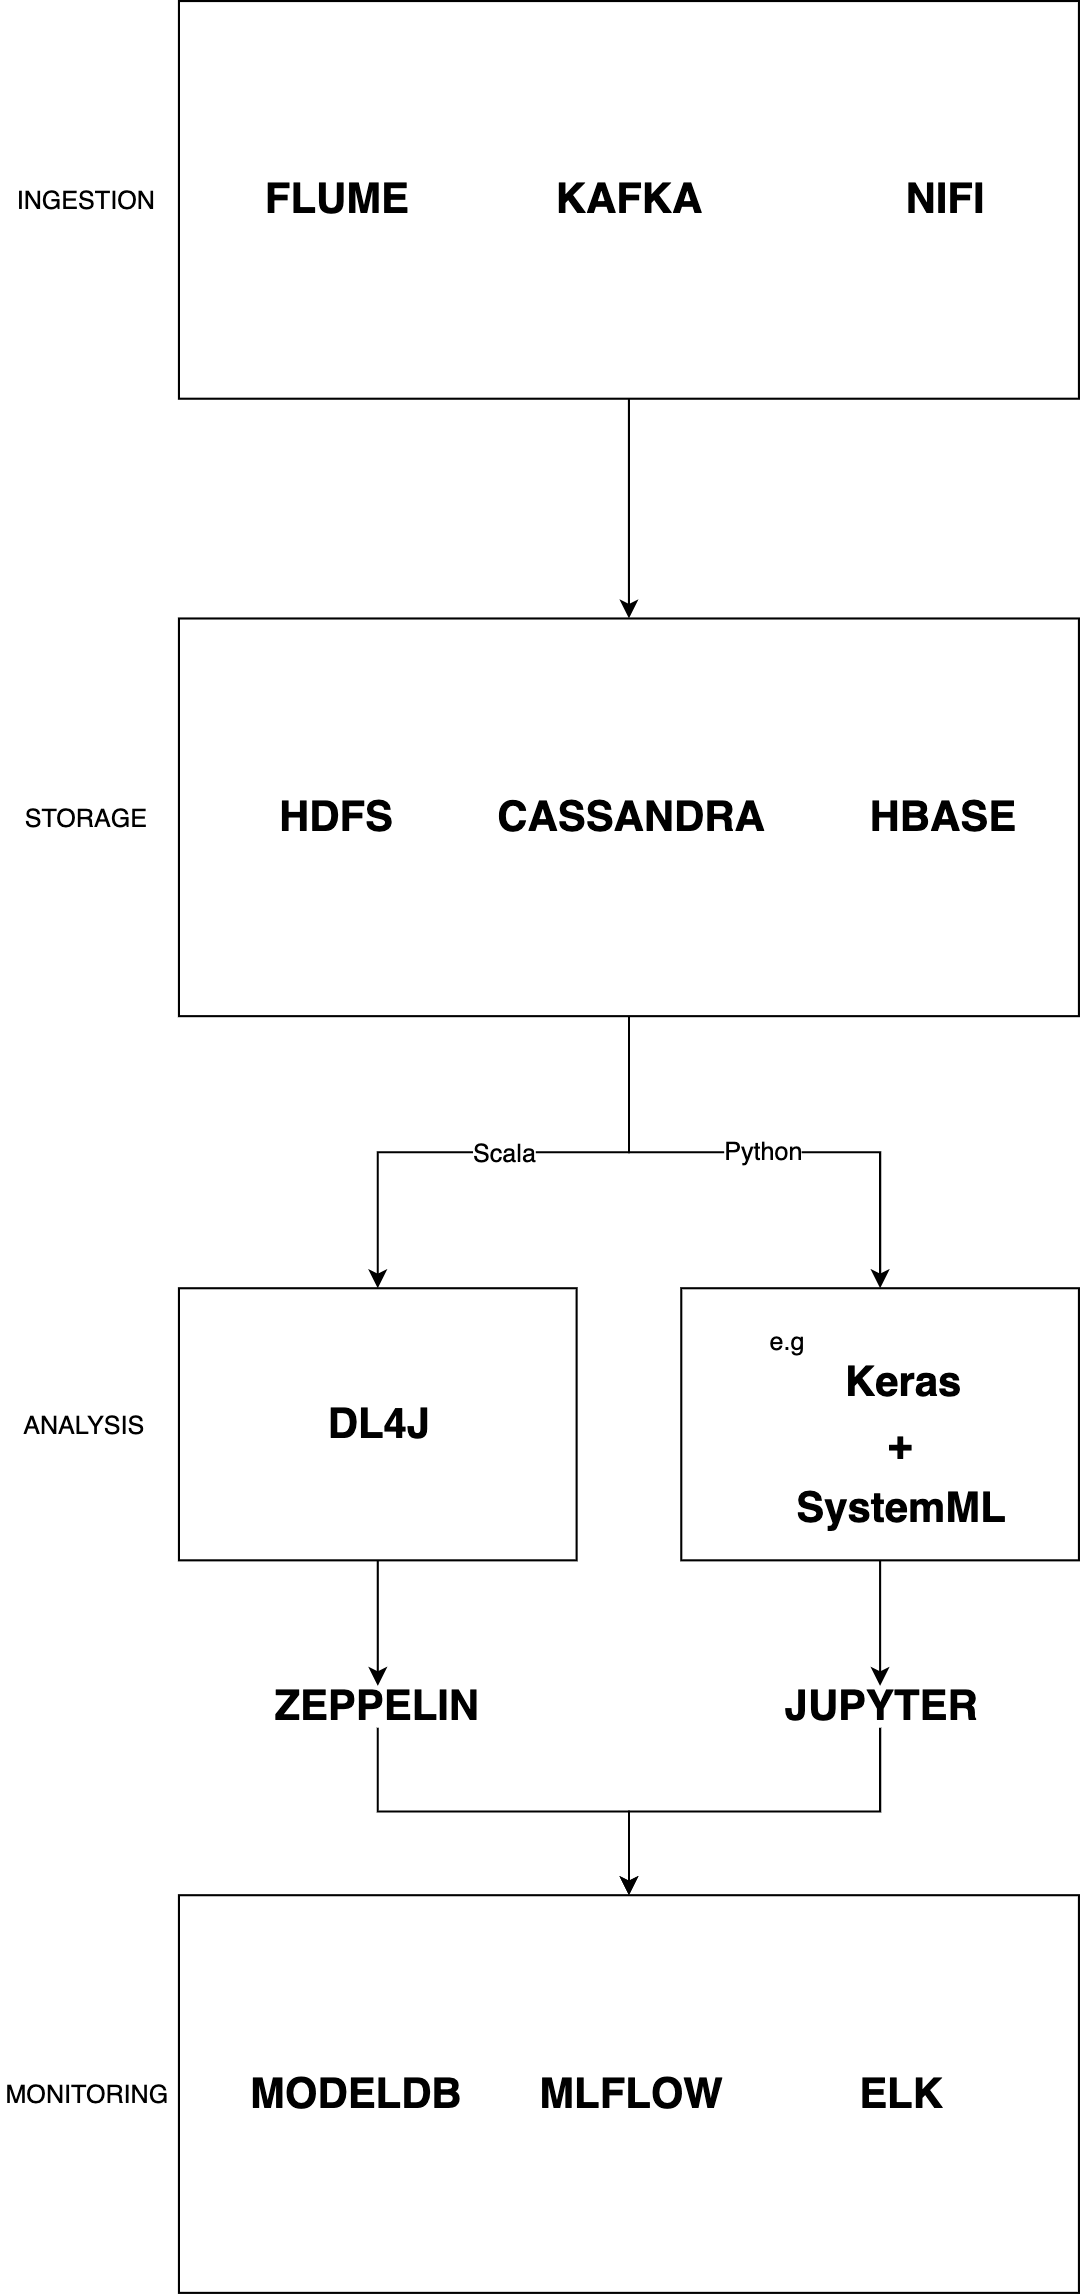
\includegraphics[scale=0.33]{images/select_flow} 
    \centering
    \caption{Example technology selection flow}
\end{figure}

We have narrowed down the number of possible technologies a lot to fulfill our requirement R2.
The recommendations here are not absolute and the user is encouraged to use the technologies they are comfortable with if they know technologies that would fit their pipeline better.
The goal of this step is to make the technology selection easier for novices by recommending technologies that have been seen to work in this domain.

The technologies that have been chosen here are the ones that we examined in the background chapter.
These choices were made mostly based on technologies that are already in use and have been through this confirmed to work in stock data environment.
We have added couple of new technologies based on their reputation in this field and how they at least theoretically fulfill the requirements that we defined in the previous chapter.
From the requirements perspective all the ingestion technologies should in some sense fulfill the requirement R5, all the storage should fulfill R6 and all the analysis part should fulfill R7-R8.

The ingestion step is the most complicated one as the format of ingested data can be almost anything and the technologies we have listed can be used as they are or with conjuction with each other.
Custom ingestion choices are also common in this field.
Our recommendation with the data sources introduced in previous section is to use custom ingestion with Apache Kafka as most of the technologies listed here have somewhat little support for HTTP based sources.
Flume works well if the data source is file or log format (e.g the sources providing excel formats) and NiFi can be used instead of Kafka if the user wants different kind of data routing management.

The storage selection is more straightforward.
HDFS works with almost any case as it has a rich development environment, but the downside of it is that it lack proper query languages at it is.
Cassandra and HBase do provide these but they both have their own use cases based on the CAP (Consistency, Availability and Partition tolerance) theorem which states that no system can guarantee consistency, availability and partition tolerance at the same time \cite{cap}.
Cassandra provides availability and is recommended to use in application where the data is fetched directly to the user and the inconsistency of data is not a problem.
HBase is the vice versa of this by promising consistency of data instead of availability.
Which one the user chooses depends on the users use case.

For the analysis, as we saw in the background chapter, Spark is the de facto environment to run distributed processing.
However, our requirement R8 limits quite a bit our options.
If the user has chosen Scala as the main programming language we recommend using DL4J for the analysis at it provides support for distributed training in Spark and deep learning models.
In the Python side the situation can be challenging in the sense that user might have to combine couple of libaries to make the models train in truly distributed manner.
Some of the de facto deep learning libraries in Python, such as Pytorch, have been designed mainly to be run on one machine.
Users can go around these limitations if the library supports exporting the models into some universal model language that can be run in distributed enviroment using other specific libraries for this.
We have included one example of this with Keras and SystemML which allows running Keras models in Spark, but as the number of possible combinations is quite large we recommend the user choosing combinations that they are most comfortable with.

After this recommend adding a language specific notebook library into the pipeline.
Zeppelin if the language of the pipeline is Scala and Jupyter if the language is Python.
This is to make the pipeline more reproducible (R4) and sustainable (R3) as the user has a way to share their experiments in more compact form instead of sharing the whole pipeline for each experiment.

Finally we have the monitoring which is somewhat optional field.
We have collected here choices that could be most useful for novice data scientist and should not require much work to integrate into pipeline, but user should pick ones based on their own needs.
Adding each should increase sustainability of the pipeline (R3) as they make easier to monitor the experiments in the pipeline and what could go wrong with these experiments.

\subsection{Implement and share}

Final two steps are implementation and sharing.
For novice data scientists, we recommend building the architecture/configuration using Docker and Docker Compose container technologies \cite{docker}.
These allow the user to develop multi-host systems in their local machine in a realistic virtualized enviroment.
We have chosen this approach, because of multiple reasons.
First, because Docker allows user to develop multi-host system in a single machine, the user does not have to rent or own multiple machines to develop the system.
This makes the development of configuration very cost-efficient as there is no costs from testing it in a distributed environment.
Second, because of the nature of docker Containers, the system becomes very easy to share and run on new machines.
This directly linked to the requirement R4.

Once the user has managed to produce the architecture and configuration in docker enviroment we recommend the user to share this docker project at this point.
At this point of the development the configuration probably includes already a lot of valuable information for new novice data scientists that can use it as a reference.
As the development is not very far at this point there is no harm sharing this as the pipeline probably does not contain much classified information.
The only way to fight the lack of information is by producing more of it and this would be a low effort way to do it.

This concludes the examination of our proposed methology. 
Next we move on to test it in practice via specific example case.

\section{Use case}

In the implementation part of this thesis we will be trying this method in a use case that reflects one possible situation that this method could be used.
Ideally, we would want multiple use cases, but because of the time constraints that this thesis has we have settle for one.
In this and the following section we will describe this use case and define how we are going to valuate the results from this use case.

\subsection{Description}

We will try the method in a situation where we have a novice data scientist that has the following background knowledge and needs.
In this fictional situation, we will call this novice data scientist as Novice A for more compact text.

Novice A has computer science background and has studied machine learning in the master's degree level.
Novice A, however does not know anything about big data pipelines and little about DevOps.
Now Novice A is faced with a problem where he is tasked in his new job at small startup that was just established to develop a system that predicts stock market prices using state of art methods.
The startup wants to use this system in the future to predict social media trends so the system must be able to handle big data from social media in the future and possibly big data from stock market if the idea works.

As the Novice A does not know anything about the stock market analysis and big data pipelines, he uses this method with the following choices.
\begin{enumerate}
    \item Novice A chooses IEX as their data source from the list of data sources as it fulfills the data needs
    \item Novice A chooses Scala as the main programming language as this is the language Novice A is most familiar with due to education
    \item Novice A chooses the following technologies:
    \begin{enumerate}
        \item Custom ingestion with Kafka for ingestion because of the data source they have chosen
        \item HDFS for storage because he its mature developing enviroment
        \item DL4J for deep learning because no other choices really exist for Scala with Spark
        \item Zeppelin for notebooks because no other choices exist for Scala and Novice A wants a way to share their results easily
        \item MLFlow for ML monitoring because there probably will be a lot of iterations to develop a working model because of the age of the startup
    \end{enumerate}
\end{enumerate}

In the next chapter we will examine more throughly the implementation step of these technologies and see what kind of challenges this selection brings.

%As we saw in the first chapter there is a lot of higher level information available about stock pipelines and the technologies they use, but as these are only high level information a lot of practicalities needed to reproduce the pipelines are left out.
%There is also a lot of good documentation about how to get started with these technologies but these methods usually are not that sustainable.
%What we want to do in the following implementation chapter is to bring this gap down by building a novice friendly pipeline that somewhat reflects what are the pipelines used in reality.

%Other important thing we want to highlight is the challenges faced when integrating the possible technologies.
%We want to show what are the challenges that novices face and provide information from this in order to prevent these adversities on happening to our possible reader.

%The pipeline will not be the best one could build for stock analysis, but the idea is more to show a way to build a novice friendly pipeline and highlight challenges that novice can face while building one.
%We will use a lot of ready made products listed in the previous chapter as we do not want to invent the same thing over again when somebody else has already done it better.
%So when we say we are building a pipeline, it is more that we are building a configuration to integrate all these pieces together.

%\section{Building a novice friendly pipeline}

%In the implementation chapter, we will build a pipeline that has two major characteristics to make them sustainable and more novice friendly;
%The pipeline will be entirely containerized using Docker and the whole pipeline can be operated using Scala.
%In this section we will go through the reasoning of these choices and how we think they solve some of the problems presented in the first chapter.

%One of the problems with stock data research was that the pipelines presented were quite hard to reproduce as they were presented from such a high level.
%This combined with quickstart tutorials which encourage to run the technologies manually from command line can make it really hard for novice users to develop pipelines that are reproducible and efficient to develop onto.
%These are usually not reproducible as they might have a lot of third party dependencies such as java which are only installed into the local computer of the user and these can be inefficient to develop onto as these might need a lot manual steps in order to run the whole system.
%To solve this we will be using Docker and Docker Compose to build containerized pipeline.

%We chose Docker as the container technology as cloud providers such as Google Cloud Platfrom and Amazon Web Services both support Docker images. \cite{awsdocker} \cite{gcpdocker}
%With Docker one can run their pipeline in local or distributed environment allowing the developer to develop their system in realistic distributed virtual environment even though they would not themselves have the resources to use actual cloud service.
%This of course fits perfectly to the needs of our target group.

%There is nothing new when it comes to containerizing a technology as this has been used as form of development for years.
%The problems come from the overall system.
%Docker images usually work very well by themselves, but when we start to integrate multiple images and technologies together the problems usually arise.
%This is due to the huge amount of different combination of technologies and the continous development of each which can break any of the integration with others.
%So each pipeline poses different problems and we try here to show what kind of problems there can be and how to solve them.

%We also want the pipeline to be developed using as little different programming languages as possible.
%This is to take away the burden of a novice data scientist to learn multiple new languages although one can assume that this kind of person has experience from for example Python.
%Although Python is very popular amongst data scientists, we chose to use Scala as most of the open-source Big Data products are build on top of JVM (Java Virtual Machine). 
%It has also a good interoperability with Apache Spark and its programming interfaces for both object oriented and functional paradigms.
%On top this, Scala offers static typing which is extremely helpful to prevent errors that can occur with long computations saving developers time and resources. \cite{scalabook}
%So we think that Scala would be the most beneficial language to use in this type of scenario.

%\section{Technology selection}

%Next we will explain what technologies we are trying to use in each part of the pipeline.
%The choices are highly based on the technologies that have been seen already in use, but there are also choices that seem promising but do not have real-life examples yet.
%Although the end product itself is not our main objective here as we want to highlight more about the challenges and the way of building this pipeline, we still want to make the system to be as realistic as possible.

%We want the system to be able to ingest normal structured stock data, but have the ability to extend to third-party metadata that can have any form and is usually unstructured.
%Because stock data by itself can already scale to gigabytes per day we want the ingestion have the ability to scale with input.
%So for the ingestion we will try to use one of the technologies that we introduced in the previous chapter: Apache Flume, Apache Kafka and Apache NiFi.
%All of these are scalable data ingestion frameworks that have different paradigms of handling data as seen before.
%For only local development these products are a bit heavy weighted, but for scalability these are necessary in order to handle massive amounts of ingested data from varying sources.

%The storage should have the ability to scale to the possible terabytes of data.
%This means that even when amount of data is enormous, the queries should be executed in somewhat manageable time.
%The storage should be fault tolerant in a distributed environment in order to ensure that the data waiting to be analyzed retains its quality throughout the wait.
%To fulfill these requirements, we will be testing plain HDFS, Apache Cassandra and, if there is time, Apache HBase.
%All of these storage formats have been developed to be used in big data environment and from these HDFS and HBase were both used in some existing pipeline.
%HDFS does not have as good as query capabilities that could be hoped for but it offers easy integrations to other technologies and a mature development environment which is perfect for novice developers.
%As for Cassandra, we are trying to see whetever it is easy to integrate with the other technologies and can it bring anything to the pipeline with its high availability features.

%For the analysis part of the pipeline, the pipeline should be able to preprocess the data for training algorithms that uses it and again the amount of data can be from gigabytes to terabytes.
%As we saw in the backgrond chapter, the current cutting edge methods for stock data analysis are deep learning methods.
%This is why we want the analysis frameworks have the ability to build and train these models without having to implement them from scratch.

%For analysis, there does not exist that many options that work well with our requirements.
%The main difficulty here is to keep our pipeline using mainly Scala for programming.
%There are two machine learning libraries that have Scala support that they promote and can be used in big data context; Apache Spark ML and Deeplearning4j libraries which were introduced in the previous chapters.
%Because deep learning, and specifically LSTM networks, is the current trend in stock analysis, the library needs to have support for these.
%Unfortunately, Spark ML does not have these natively as the writing of this, so that leaves us with only Deeplearning4j.

%Because building and demonstrating data analysis applications can be a time consuming and complex job, data science community has adopted the usage of Jupyter notebooks when implementing data analysis in Python.
%For the same reasons, we will be integrating Apache Zeppelin notebooks into this pipeline as these have a support for Scala programming language and allow submitting applications to Spark cluster.
%This is to help with reproducibility of models developed by the users.

%Finally, we have the monitoring of the pipeline.
%We want to allow the novice data scientist to have a simple and intuitive way to manage and monitor the the state of the whole pipeline.
%The main goal is to give the data scientist an ability to notice errors in the pipeline as soon as possible this way preventing the errors to possibly escalate to the latter parts of the pipeline.
%We would also want to allow good tracking on progress of machine learning model development in the analysis stage to give the analysist tools to track the results of training.

%To monitor the machine learning model development we will integrate the MLFlow tracking into the analysis phase.
%This is done by implementing a separate tracking server to allow this process scale separately from the actual analysis.
%Thus also enabling responsive tracking UI usage.
%If there is time, we will also try to develop a global ELK stack which was described in the previous chapter to give global monitoring on the entire pipeline.

\subsection{Analysis of results}

%The main objective of our practical research is to show that the problems described in the first chapter do exist and provide valuable information to novice data scientists on how to build reproducible and sustainable pipelines without a lot of resources.
Now that we have seen our specific use case, the next question is how are we going to test whetever the methology actually helped?
%So the question is, how do we validate the results of this empirical part?
We will be using qualitive analysis focusing on the requirements that we have set to this method. %reproducibility of the experiments in the pipeline, sustainability of the pipeline and how novice friendly the pipeline is.
So we will be examining the sustainability of the pipeline, the reproducibility of the pipeline and novice friendliness of the pipeline, but we will also discuss about traits that big data pipeline should have e.g scalability.
%For these we will use same definitions that we have used to this point.
%These are not mutually exclusive terms as, for example, a pipeline that is easy to reproduce has a lot of same characteristics as novice friendly pipeline.


%By reproducibility of the experiment, we refer to the amount of work and information needed to reproduce the pipeline itself and run an experiment on it.
%This is related to the one of the problems with many stock analysis papers that report their pipelines but from a very high level making it hard for example novice data scientists to replicate the experiments.
%Here, however, we will not be focusing on the amount of information published, but instead we will focus on how much manual work the user must do to run the pipeline.

%We will be using the term "sustainability" again to mean the effort needed to develop the pipeline in the future.
%Developing here can be divided into multiple parts, but we use it to refer the process of continuously building new features and keeping the components up to date.
%This is related to the problem that there is a lot documentation that shows how to get started but these instructions usually do not make the system sustainable to develop onto.
%We will be focusing on the aspect of how much work is needed to upgrade components in the system and how does the system support new features.

%Finally, with novice friendliness we mean how much does the user has to know about underlying technologies in order to start their own experiments.
%We will be also using this term to analyse how much resources such as money is needed to run the experiments as this is something usually novice data scientists do not have much on their disposal.

We will be comparing the pipeline with two different pipelines using these qualitive metrics.
Because of the scarcity of possible points of reference the pipelines have a bit different purposes, but we are more interested how do these pipelines compare with our metrics.
We have picked one pipeline from the academia and one pipeline from the industrial side.
The pipelines are depicted in very high level which can make it hard to make any reasonable deductions, but given the scarcity of data available it is the best we can do.
We are more interested in how they are run than the actual components that they are made of but to give a better picture we also introduce the architectures.

% for screenshots
\begin{figure}[ht!]
    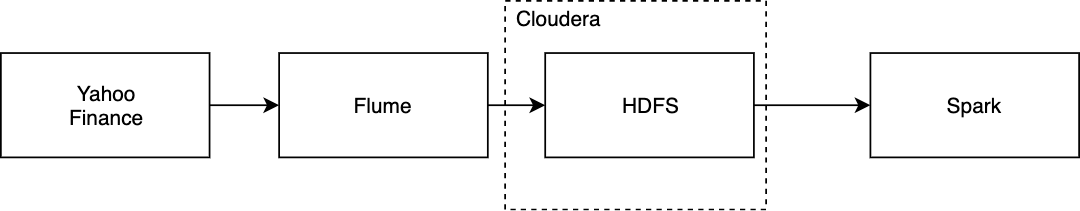
\includegraphics[scale=0.50]{images/example1} 
    \centering
    \caption{Simplified architecture of the academic pipeline}
\end{figure}

The pipeline we have picked from academia is the pipeline proposed in \cite{peng}.
The reported architecture in the paper is recaptured in Figure 4.1.
From the paper we know that the system was ran locally using local Cloudera instance.
Python was used with PySpark as the programming language and the pipeline ran normal machine learning models.
Although this information is not much, we can use it to make some observations on our system.

% for screenshots
\begin{figure}[ht!]
    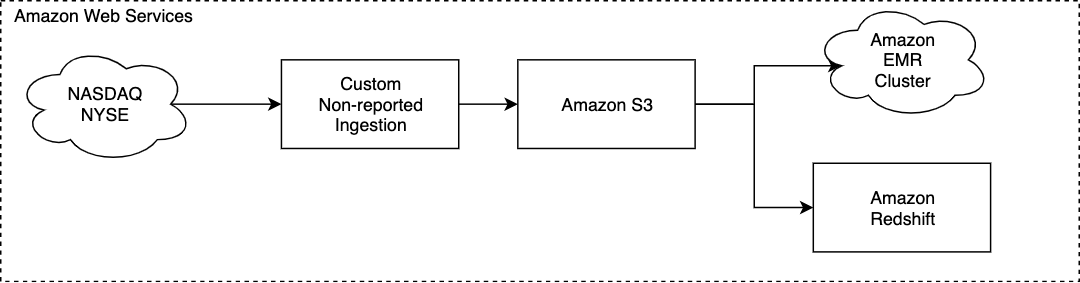
\includegraphics[scale=0.50]{images/example2} 
    \centering
    \caption{Simplified architecture of the industrial pipeline}
\end{figure}

The industrial pipeline that resembles the most of our pipeline here is the pipeline recaptured in \cite{snively}.
The high level architecture shown is presented in Figure 4.2.
What can be seen in the architecture is that we do not know much about the parts of programs that analyse the data.
Amazon EMR can be used to run almost many different big data frameworks but given that they report using it to analyse data it is higly likely that they are running multiple Spark clusters there.
But what we do know for sure is that the system is run on Amazon Web Services in large scale and we can use this to analyse our own system from the perpectives that we listed above.


We will also be quickly reflecting on the reported challenges.
We will question whetever these are significant in the sense that they could happen to any novice data scientist and is the cause of these challenges in this methology or could they have been avoided using other methods.
%We will be also analysing whetever these challenges could have been avoided and what was the root cause of these challenges.

This concludes our chapter on the proposed methology and its planned usage in the empirical part of this thesis.% were we examined and reasoned the plans we have for the empirical part of this thesis.
In the next chapter we will report the process of the implementation this in the depicted special case and see what kind of challenges were faced during it.


%After the we have the implemented pipeline, we need some ways to measure whetever our system fulfills the requirements it has been given and how does it compare with other software that might be as good as it.
%In this section we will introduce the measurements that we will be using in the chapter 6 after the implementation.
%Some of these are quantative such as the performance metrics, but these usually give very shallow view on the system.
%Because of this we will be using more qualitive methods in order to grasp the actual benefits of the pipeline.

%Our focus with the qualitive metrics is going to be on how easy the pipeline is to develop onto and how well the user can monitor changes in the pipeline.
%These are usually important factors when continuously developing a system and can affect greatly when new developers are choosing what pipelines to use.
%This also includes how automated the processes in the pipeline are and does developing and deploying the software require excessive amount of manual work.

%Some quantative metrics are taken in order to asses the fitness of the pipeline for any kind of development where it is important that iterations of the software can be swiftly build and that the whole service can run comfortably on the developers machine.
%Namely for these reasons we will examine the memory consumption of these services on a normal developing machine.
%Other quantative statistics that we can examine are processor usage, network usage and disk usage which, although not as restricting as the memory usage, can tell a lot about the performance of the system.
%For these metrics, we will be using Dockers native tools, and especially the command 'docker stats', to measure the containers usage of resources.

%As there will be a bit different pipelines with different technologies, we can get results that can be used to compare components with one another.
%This would give the reader better information and alternatives on what technologies should they could choose for their own project.
%Now we move on to the implementation chapter where we examine more closely what was done during this thesis.

% TODO: MOVE

%For this thesis we have chosen to use data from IEX API which was an open API until 30.09.2019 when the company decided to close this in order to capitalize with the closed API which free plan is in the table.
%This data is from the 5 year interval between 2014 and 2019 and the relevant values that it contains are opening prices, closing prices, highest prices, lowest prices and volumes.
%In order to test freely with this data, we will implement a simple server that serves this data into our pipeline.

 
\chapter{Implementation}
\label{chapter:implementation}

%You have now explained how you are going to tackle your problem. 
%Go do that now! Come back when the problem is solved!

%Now, how did you solve the problem? 
%Explain how you implemented your solution, be it a software component, a
%custom-made FPGA, a fried jelly bean, or whatever.
%Describe the problems you encountered with your implementation
%work. Sometimes the content of the environment chapter is combined
%together with the implementation chapter.

In this chapter we will introduce the software created for this thesis and the challenges faced while developing it.
This chapter is divided into two parts.
In the first part we will examine technically what was the end result while quickly commenting on some of the choices that can be seen in the final architecture.
Because of time constraints and challenges during development, there were some parts such as HBase as a storage which we could not develop.
These challenges are explained in the latter part of this chapter and we continue with them in the following evaluation chapter.

\section{Overview}

In this section we will explain the practical application that was developed.
We start by addressing some of the deadends that lead to the final pipeline to give reader a clearer view what changed in practice after the previous chapter.
Some of the reasoning why some of the technologies were prioritized leading to not being to test every technology is presented here but more in-depth look at for specific integrations and problems will be examined in the next section.
Finally in the section 5.1.3, we introduce how the pipeline can be run with any novice data scientists local machine.

\subsection{Dead-ends at the start of development}

Two technologies that were mentioned in the previous chapter were eliminated at the start of the development of each.
These were Apache Flume and Apache Cassandra.
As both seemed to lead to a dead-end in the development and there existed seemingly better alternatives than these, focus was moved to other technologies.

Apache Flume was supposed to be used as a component in the ingestion step, but due to its charasteristic of being mostly aimed at data which could be fetched in log form, it could not be used with the REST APIs that most of the data services use.
Flume also did not seem to have any native ways to connect to storages such as Cassandra.
There exists some ready-made solutions for this, but these were unmantained and seemed possible dead-ends.
This is why Flume was ruled out.

Apache Cassandra was dropped from the development mostly because integrating it with other services would have required a lot of extra work. 
Further examination of Cassandra also showed that Cassandra is not very good choice for this specific purpose that we want to use it for.
Cassandra is known for its ability to write enormous volumes of data, but when it is time to read from the storage the task becomes non-trivial.
Reading from Cassandra is based on the Cassandras query language, CQL, which allows somewhat efficient queries but you have to define these high perfomance queries at the time you create tables for data. \cite{dronavalli}
Because our pipeline should be used mostly by analysist who can have varying queries into the storage this raises a challenge for future development.
This is why we decided to discontinue with Casssandra.

\subsection{Final Architecture}

% for screenshots
\begin{figure}[ht!]
    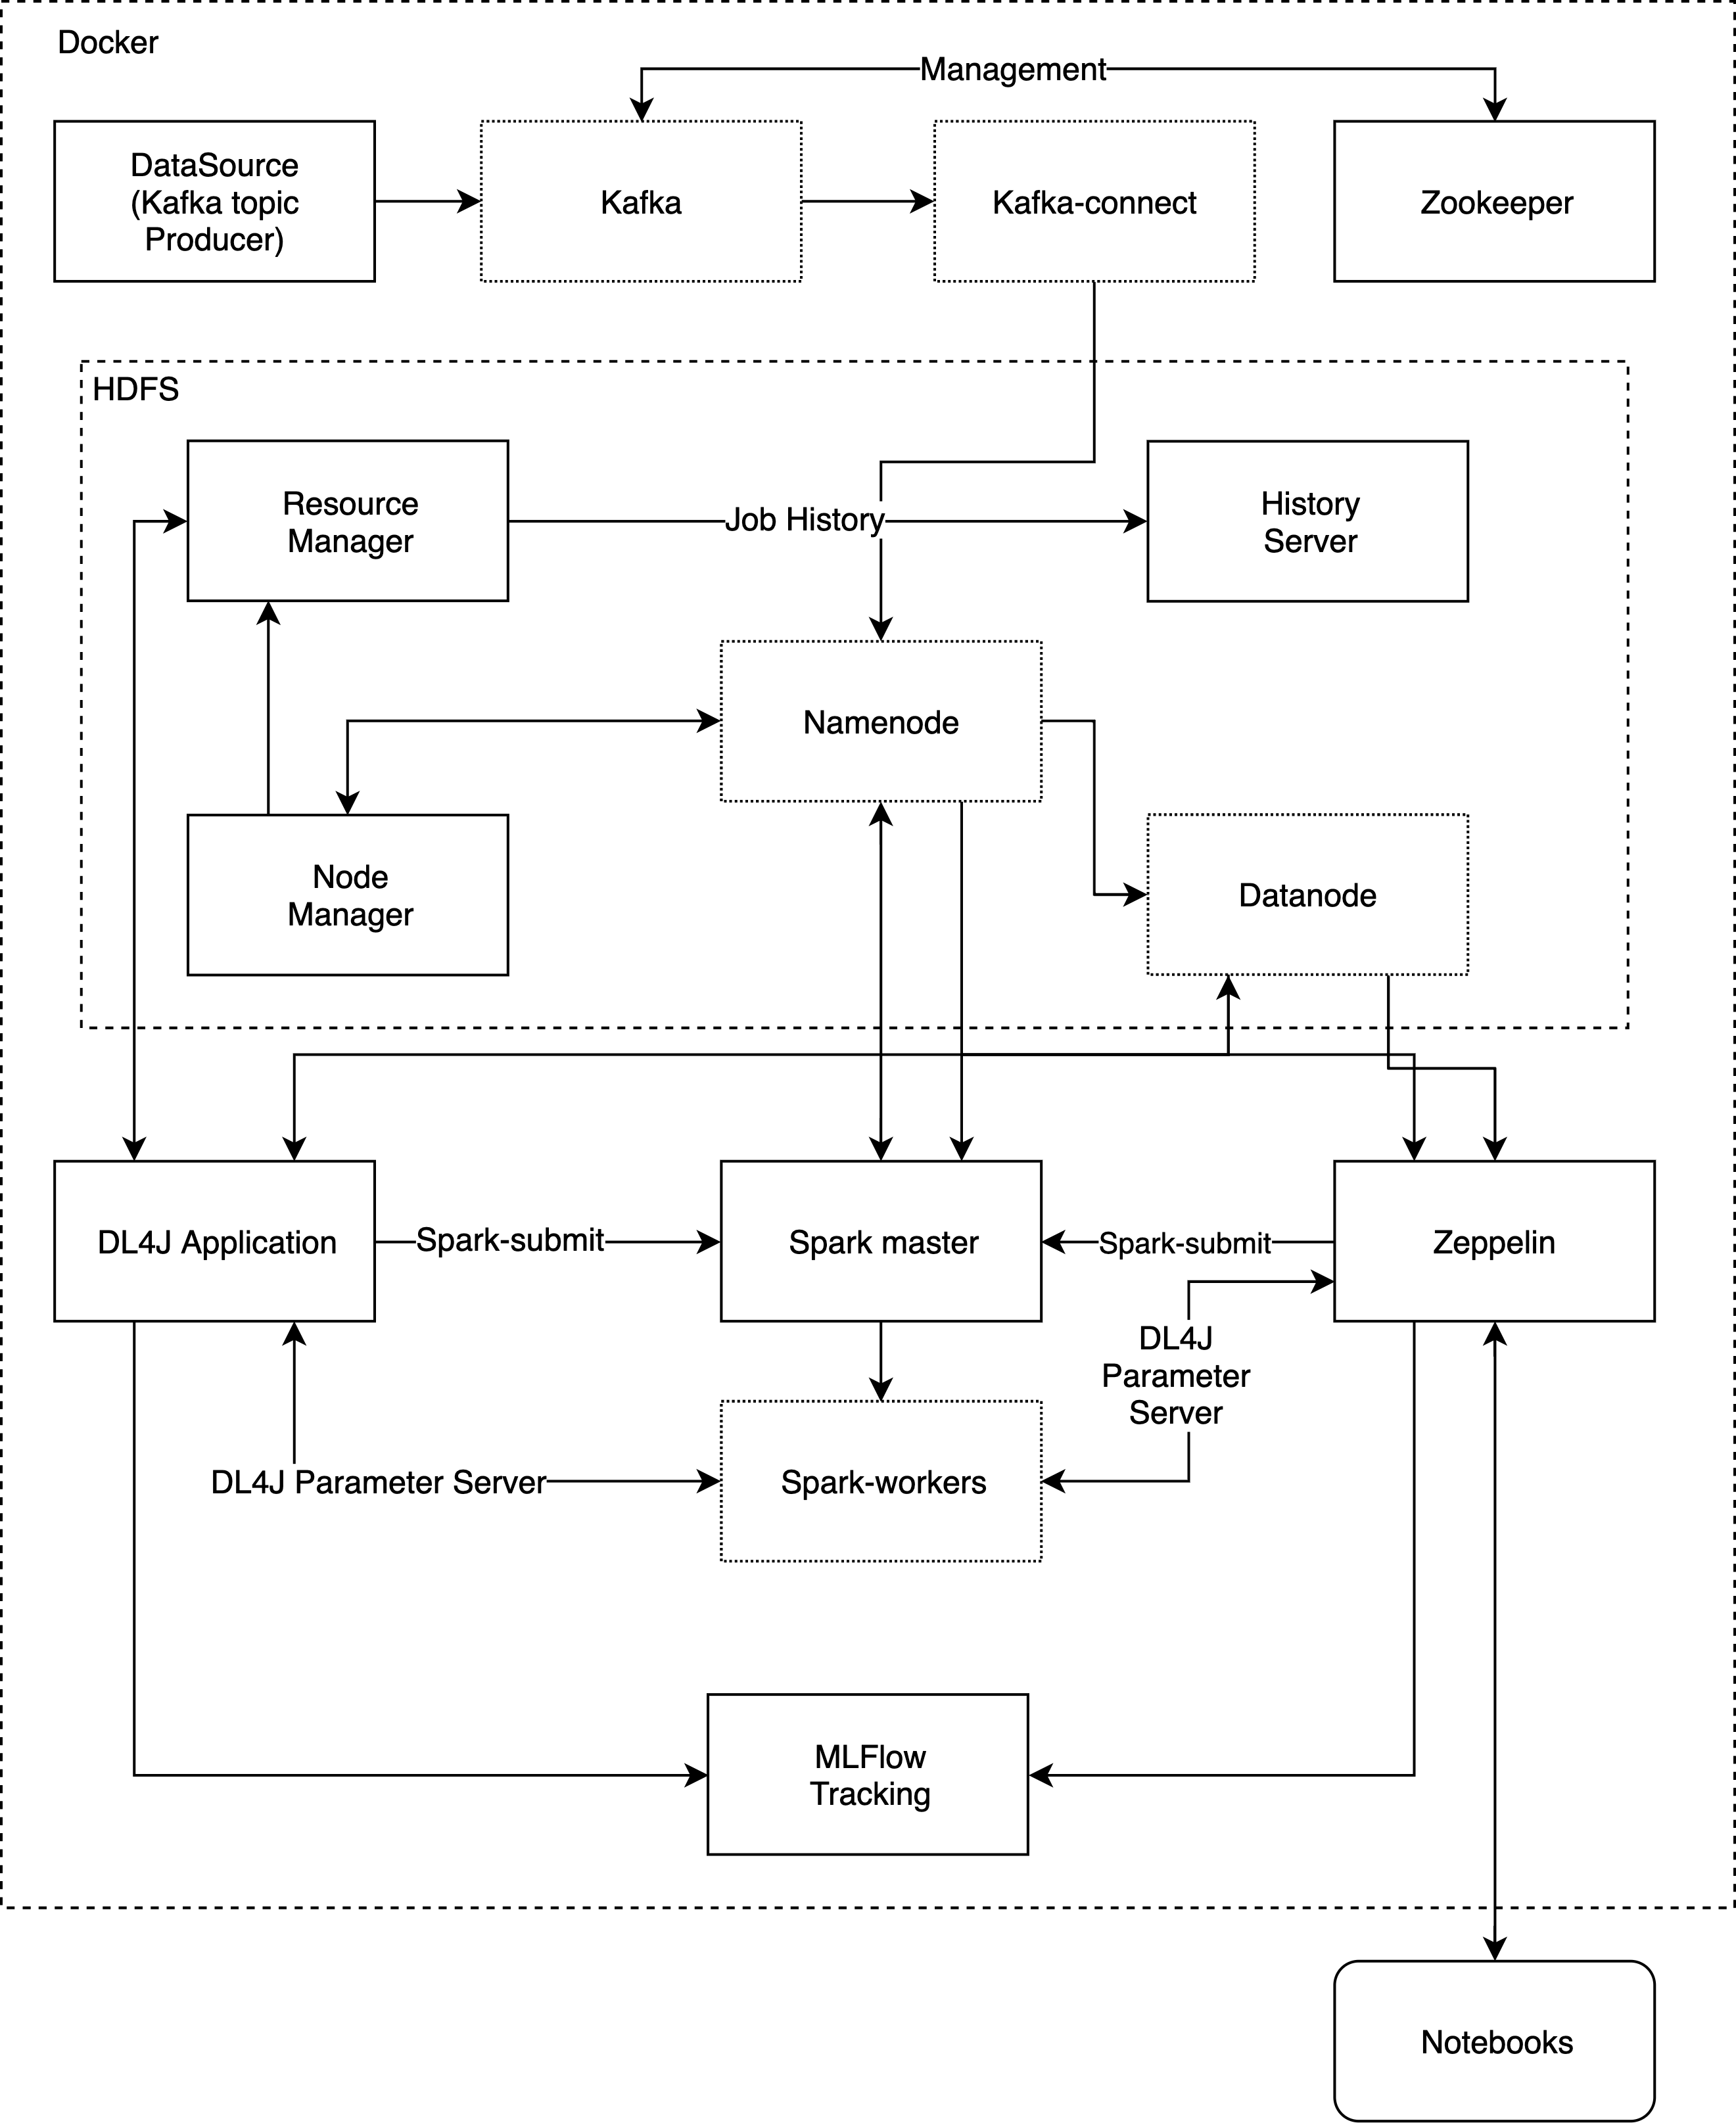
\includegraphics[scale=0.20]{images/architecture} 
    \centering
    \caption{Final Architecture of the implementation section}
\end{figure}

The final architecture can be seen in the figure 5.1.
The figure presents the main dependencies between the components each arrow usually presenting the flow of data in the system with labels sometimes added to clarify better the relation.
In the figure each solid rectange represents one actual server with its own process with the exception of rounded rectange to represent notebooks that are stored into the local file system.
In the case of this thesis these servers were virtual machines but theoretically the system could be run with right configuration with multiple physical machines that are in the same network.
Rectangles with small dashed lines such as with the spark workers represent that the server can have easily more than one instance allowing horizontal scaling.
The longer dashed lines here represent bigger entities such as the HDFS cluster to make the figure more readable.

The pipeline starts from the data source that acts as the kafka producer.
It reads the data from a source, in this example case from JSON files, and produces the data into a kafka topic. 
It also creates the needed kafka topics on startup using Kafkas admin API.
Although most of the kafka documentation recommends using the command line client, this did not seem production-ready way to do this as this decouples the topic creation logic from the actual producer and would need excessive scripting in order to automate this process which did not seem as maintainable as the admin API approach.
This is why admin API was used in the data source server. 

Then we have Kafka which is integrated into HDFS cluster with Kafka Connect HDFS 2 Sink connector which is a component made by Confluent.
This acts as a kafka consumer and listens to the topic that the producer defines.
Connect can be scaled and contains some basic configurations that can be used for example to define the format in which the data is stored into HDFS.
We have chosen JSON as the format which the data is stored but Apache Avro is also an option.
Other notable configurations that can be used to tweak the pipeline are the rate in which the topic is consumed into the HDFS and schema validation.

In the middle of the pipelin is the HDFS cluster.
In this cluster there is the normal HDFS cluster with namenodes and datanodes which can be accessed to directly read the data.
There is also a YARN resource management on top of this which can be used to for better manage IO routines in the cluster.
This consist of the resource manager, node manager and history server nodes, that can be used as an alternative route to access data.

The HDFS cluster docker containers, as well as the containers for Spark cluster later, are a work of Big Data Europe project.
The Big Data Europe is project funded by European union which one of the goals is to produce open-source tools for big data development without the need to use closed softwares.\cite{bigdataeurope}
As these containers were the most maintained hadoop containers at the moment of writing this, they are were the best option for this case, but they brought a couple of problems which we will examine later.

\begin{table}[! htbp]\centering
    \caption{Storage and ingestion components versions}
    \begin{threeparttable}
        \begin{tabular}{|c|c|c|c|c|c|c|} 
        \hline
        & Hadoop & Kafka & Kafka Connect & Zookeeper \\ \hline
        Version & 3.1.1 & 2.3.0 & 5.2.1 & 3.5.5\\
        \hline
        \end{tabular}
    \end{threeparttable}
\end{table}

In table 5.1 we have gathered the versions of the technologies used in the first half of the pipeline.
Most are the newest versions of each software at the writing of this.
The version of hadoop is specially tricky as its clients are used in multiple parts of the pipeline coupled with other software libraries which have support for only some of the older versions but do not complain if used with the newer one.
This is why there can be other versions than this in the pipeline e.g in the spark cluster, but as they do not currently cause any visible errors and due to the time constraints that this project has, the versions can mismatch for now.

After the HDFS cluster comes the analysis part of the pipeline which has Spark cluster in the middle and two options to run analysis code on it.
The application part allows writing production grade scala applications that can be run like any normal scala spark application.
The Zeppelin is a Apache Zeppelin instance which allows writing and running notebooks that can be saved into local file system for distribution.
Both approaches submit the spark application to spark using spark-submit script and the DL4J communicates with itself with its own parameter server.

In default case, the spark application first preprocesses the json formatted data and saves this back to HDFS as csv files.
In this process, it normalizes the data and appends labels to it that in our example case is just values 1 and 0 whetever the value of stock grew in n-days after the datapoint or not respectively.
The data is stored back as a CSV file because DL4J is quite picky about the data format that it accepts and does not have simple default way of transforming spark DataFrames with sequential data to the Dataset format that it internally uses.
After this the data goes through the training and evaluation pipeline which logs its parameters and results into MLFlow server where user can monitor the process of their different experiments.

\begin{table}[! htbp]\centering
    \caption{Analysis Software versions}
    \begin{threeparttable}
        \begin{tabular}{|c|c|c|c|c|c|c|c|} 
        \hline
        & Spark & Scala & Java & DL4J & sbt & Zeppelin & MLFlow \\ \hline
        Version & 2.4.3 & 8.x & 2.11.12 & 1.0.0-beta5 & 1.26 & 0.8.1 & 1.2.0\\
        \hline
        \end{tabular}
    \end{threeparttable}
\end{table}

In the table 5.2 we have collected the versions of different components in this part of pipeline.
Almost all of them are the latest releases of each technology at the time of implementing with the exception which is the version of Scala.
Currently, the latest version of Scala is 2.13.
Spark mainly supports scala 2.12, because as of 2.4.1 version of spark, the version 2.11 of scala is deprecated and there is still no support for 2.13.
However, Zeppelin does not support Scala version 2.12 so the only version of Scala that still works with all of the latest releases of these two technologies is 2.11 which is why it had to be chose for the version.
Java is still version 8 which is already at its end of life stage, but it was used as it is currently the safest way to ensure that your code runs correctly.

\subsection{Usage}

The initial idea of the project was to provide modular design for the pipeline where the user can cut and paste the technologies to the pipeline making it easy to produce multiple different pipelines for comparison.
That is why the there is a initialization script called pipeline.sh.
This is a command-line interface that asks user what technologies they want and builds a docker-compose file into build folder with all the necessary files.
Sample usage is depicted in the figure 4.2.
Only thing user has to do before running the script is to download manually the Kafka Connect component from confluent website and copy its content to a location noted in the project readme. 
This step is mandatory because unfortunately Kafka Connect did not have public distribution that would have allowed access without authentication.
If this component is missing during the build, the initialization script notifies user about this before continuing further.

After the initialization, using the software is the same as with any other normal docker-compose project.
Users can copy the contents of the build folder as the base of their own project or use it as it is.
The project can then be build with "docker-compose build" command and run using the command "docker-compose up".
After this as there will be over 10 containers running simultaneously, tools such as lazydocker are recommended for proper management.

When the containers have finally finished the startup procedures, every services user interface can be found in their default ports in localhost.
The ports needed to be open to this happen, can be found in the docker-compose.yml file.
To start analysing data, the user has to only open localhost:8090 where Zeppelin notebooks are running.
In the project there exists an example notebook that implements a simple LSTM model.
To run this example on spark cluster user has to first manually set two configurations in the spark interpreter menu that can be found under interpreter settings in the user interface.
The value "master" must be set to "spark://spark-master:7077" in order to let the zeppelin use the cluster instead of local spark client.
Also in the dependencies has to be added "org.apache.commons:commons-lang3:3.6" in order to have common versions in the zeppelin machine and in the cluster.
The reason for the manuality of these tasks will be discussed in following sections.
After this the user has to only run the cells in the notebook and the result will be saved into HDFS.

To add third party dependencies to the notebooks such as the DL4J library, the "spark.deb" syntax in notebooks is encouraged as this is the best way to preserve the dependencies for possible distribution of the notebook.
This way the notebook is as independent of its environment as it can be.
It is currently also the only way to preserve these if the container happens to be destroyed. 
Reasons for this will again be discussed in following sections.

\section{Adversities during development}

Most of the time during development went to trying to integrate these services with each other.
The reason for this was mostly features that were not documented well and other misshaps such as bugs that happen when integrating two services that are not that common together.
There was a lot of unique problems that did not have any documented solutions on the internet which made solving them very time consuming.
In this section we will be going through the ones that took most time to solve and present the solutions at high level to these problems.
More precise technical problems with their solutions can be found in this thesis' git repository that contains all the practical results.

\subsection{Kafka-HDFS integration}

Integrating Kafka topics to HDFS proved to be a non-trivial task.
Unlike products like Flume, Kafka does not have any build-in sinks that would allow easy integration of different services.
So the developer is left with the task of filling this hole.

The requirements for this component are also non-trivial, as it should be able to scale with the kafka and the HDFS cluster.
So in order to not introduce a bottleneck to the pipeline and to do this with time limits that this thesis has, a ready-made solution was necessary.
Previously, a good solution to this has been Linkedin's Camus API, but this was phased to Apache Gobblin in 2015. 
The problem with Apache Gobblin, however, is that it is not the lightest tool and it can move data only to Hadoop system.
That is why if we were to change the HDFS storage to try some other storage option, the Gobblin should be entirely changed to something else.

Technology that solves these problems is Kafka Connect. 
Kafka Connect acts like a sink plugin to Kafka.
Unlike with Gobblin, developers can download only the sink they actually need instead of sinks for every possible case.
Because Kafka Connect has sinks for most major big data storages in the market, user is not constrained as much to Hadoop ecosystem like with the Gobblin.

The downside is that Kafka Connect is clearly Confluent product although it is open-sourced and free.
Confluent has its own platform that it promotes as open-source event-streaming platform that can be used as a enterprice solution. 
This is why most of the Kafka Connect documentation is only about how to use it on top of this Confluent platform, although it has capabilities to run independently.
This lack of good documentation introduced some obstacles for integrating this component between Kafka and HDFS especially when it came to installing and running the component.

Setting up the Kafka Connect was not that easy as it does not offer much monitoring in itself.
This means that as developer you could only see if the whole system worked or did not from HDFS management console.
If only some configuration was not right, Connect would only log this as an minor error in the stderr and continue running like nothing had happened although no data was flowing through it.
This made debugging the connection surprisingly difficult, but after all the configurations were in place the component worked as it should throughout the rest of the development.

\subsection{Apache Zeppelin dependency management}

Major problems came when the development reached to the point of adding DL4J dependencies to the Zeppelin instance.
Zeppelin has multiple ways of adding dependencies and the main way that is defined in its documentation is by its dependency UI that is located in its interpreter settings panel.
This again saves these settings into interpreter.json file which is a normal JSON configuration file.

At the start of this development in order to remove the manual step of adding dependencies and other settings, we tried to save this interpreter configuration file between container restarts.
This worked with every other setting except dependencies.
Dependencies would conflict for unknown reasons and and the error message would change per restart.
Sometimes by mere luck the dependencies would build correctly for a certain amount of time but then fail again.
This would be easy to debug if Zeppelin would be a normal maven project as it is.
But with ready-made containers there did not exist such an option.

Apache Zeppelin has official container which were used, but this had to be extended in order to have custom spark-submit client because the versions on spark cluster would conflict.
When thought afterwards, the whole zeppelin container probably should have been build from scratch as this would have allowed better dependency management with maven.

\subsection{DL4J sbt project}

The DL4J application instance without Zeppelin is build with sbt.
sbt is a build tool developed specifically for Scala applications and this why it was also chosen for this project.
DL4J's main build tool that the documentation is build around is maven because it is a Java library, but it has its own sbt example in their project repository.
This, however, turned out to be highly outdated and caused developing problems.

To have third-party dependencies added to a spark project there are two possible ways to implement this.
First one is using the spark-submit scripts flags to define maven repositories.
This was first tried but it only lead to dependency conflicts and other bugs with ivy dependency management that the script uses.

The alternative and more manageable way is to build the whole application into so called fat jar, which contains all the code to run the application including the third-party dependencies.
This is what the outdated sbt example did so we opted to update this example to work with newer versions of sbt and sbt-assembly which is a plugin needed for building fat jars on sbt.
To make the example project work, we migrated it from sbt version 0.X to sbt version 1.X syntax. 
The migration of general syntax was relatively easy, but with the newer version of DL4J library, a new merge strategy had to be written for sbt-assembly.
Merge strategy is what sbt-assembly uses when it encounters duplicate files during the building process.
Writing a updated merge strategy for DL4J was not a trivial task as the strategy that was usually suggested did not work in this case and lead to errors in runtime.
After quite a bit of trial and error, we thankfully managed to create a merge strategy that did not throw away necessary files needed at the runtime.

\subsection{Running the application in Spark}

Now we move on to the problems that were really hard to debug when the problems in the previous two subsections were persisting at the same time.
When running a Zeppelin task on Spark and the program receives error, Zeppelin correctly logs the stack trace from Spark workers stderr.
What it does not do, is logging the the whole stack trace but only the two to three first errors.
This made it seem like the error was a some upper level error when instead the actual error that happened in lower part of the stack.
This was resolved by noticing the full stack when the application was run on application server.

After this, the next problem was that Intels mkl-dnn library did not seem to be in the classpath of DL4J subdependency library javacpp.
This is the code that is responsible of allowing the java code to use high efficiency feature of C++ language.
This of course did not have any clear solutions online except some vague conversation logs about possibility of glibc missing in the parent OS and by accident this turned out to be the exact problem in this case too.
The Spark worker docker container, which was a result of the Big Data Europe project, was build on top of alpine linux image which has phased out to use musl libc library instead of glibc.
There exists tools that can be used to install glibc to alpine instance and we tried this, but after multiple errors in multiple different attempts to install the library, we opted out to fork the docker image to use debian based image.
This resolved all the problems that had been until this point and the application finally compiled in worker machine.

The problems after this did not cause the application process on worker to crash but were logged into worker machine while the process continued to run.
These were somewhat minor but laborous problems such as allocating enough disk for /dev/smh shared memory implementation and opening and defining right ports for DL4Js parameter server that handled the parameter update logic.
Once all of these were fixed, the next problem was that the training process in spark did not finish at all and seemed to go into a state of infinite loop without giving any errors on the driver logs.
This seemed like a dead-end until we noticed that a spark job before this had silently failed.
It seems that the DL4Js training code was beforehand trying to temporarily save the data into hdfs and this failed as something went wrong.
This step in the process could be skipped with configurations and after this the model training process finally succeeded.

The final problem we faced was a randomized index out bounds exception.
Raising the number of epochs we noticed that this occured at random, and unlike the previous errors, this seemed like a error in the library.
The code that raises this error handles parallel code so if we were to make conjectures from this it would seem like there would be an error with shared memory access in some part of the asynchronous code.
However at this point, the time allocated to this project was already running out so we could not confirm this definitely.

Now that we have seen what we were able to implement during this thesis we move on to evaluate the quality of this software.
We will also discuss more about what went well, what went wrong and what could have been done better.

\chapter{Evaluating the results}
\label{chapter:evaluation}

%You have done your work, but that's\footnote{By the way, do \emph{not} use
%shorthands like this in your text! It is not professional! Always write out all
%the words: ``that is''.} not enough. 

%You also need to evaluate how well your implementation works.  The
%nature of the evaluation depends on your problem, your method, and
%your implementation that are all described in the thesis before this
%chapter.  If you have created a program for exact-text matching, then
%you measure how long it takes for your implementation to search for
%different patterns, and compare it against the implementation that was
%used before.  If you have designed a process for managing software
%projects, you perhaps interview people working with a waterfall-style
%management process, have them adapt your management process, and
%interview them again after they have worked with your process for some
%time. See what's changed.

%The important thing is that you can evaluate your success somehow.
%Remember that you do not have to succeed in making something spectacular; a
%total implementation failure may still give grounds for a very good master's
%thesis---if you can analyze what went wrong and what should have been
%done. 

 %At this point, you will have some insightful thoughts on your
%implementation and you may have ideas on what could be done in the
%future. This chapter may be combined together with the evaluation
%chapter. All the new insights and findings are given here!  This
%chapter is a good place to discuss your thesis as a whole and to show
%your professor that you have really understood some non-trivial
%aspects of the methods you used\ldots

In this final chapter before conclusions, we will be examining the pipeline which we build in the previous chapter.
We start with basic perfomance metrics that were briefly introduced in section 4.4.
Then we move on to evaluate more management side of the pipeline and finally we end this evaluation with general discussion what could have been done better and what choices possibly turned out to be detrimental.
Finally we close this chapter with a section were we briefly list possible improvements that could still be made to the current pipeline, but could not be done with the resource and time restrictions that this project has.


\section{Perfomance metrics}

The following metrics were taken in a machine that has a Windows 10 as parent operating system, Intel Core i5 2500K processor and 16GB of DDR3 memory.
The docker version that the code was run against was 19.03.2 and it had 3 CPU cores and 10GB of memory as its use.
Not all of these resources were needed, but this was done to in order to, for example, remove the factor of running out of memory that caused inexplicable errors.
These were tested only in one machine which would usually no be enough to make any kind of actual inferences but because the code is run in a containerized environment the role of underlying hardware becomes less important.

\begin{figure}[ht!]
    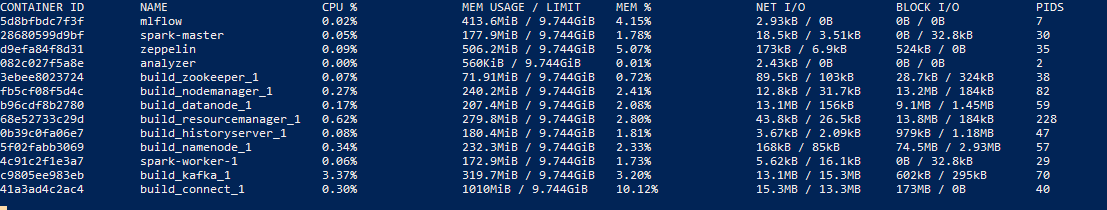
\includegraphics[scale=0.45]{images/memory1} 
    \centering
    \caption{Resource usage in idle state}
\end{figure}

The resource usage in idle state after the initial data has gone through the pipeline and stored into HDFS can be seen in the figure 6.1.
The figure is the output of the "docker stats" -command.
While inspecting the names of each container one can trivially map these into corresponding components in the architechture figure in section 5.2.
Clarifying the most ambigous namings, the "analyzer" container refers to the standalone DL4J application and build\_connect\_1 refers to the Kafka Connect instance.

The total memory usage here was around 3.8GiB of memory.
This seems to match with the fact that most of the components run on top JVM and we did not have the time to optimize each components garbage collection. 
This is partly because components such as the Kafka Connect, which had a notably large memory usage, would silently fail if not enough memory were offered.
Additionally, this would have probably lead to premature optimization.
For future improvements of the accessibility of the pipeline, this would be a great place to start.

Processor usage in idle state was minimal and did not have any notable jumps except a bit higher usage for Kafka.
The other statistics did not have any notable deviations that would affect greatly on the usage of the pipeline. 
Minor thing to note is that the DL4J application instance is not running actively during these results as user usually are not using both it and the zeppelin instance simultaneously.

\begin{figure}[ht!]
    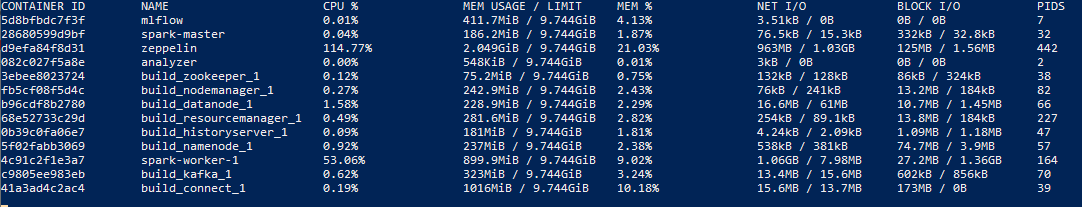
\includegraphics[scale=0.45]{images/memory2} 
    \centering
    \caption{Resource usage in preprocessing state}
\end{figure}

In figure 6.2 we have the same statistics while the zeppelin code is trying to preprocess the data in order to feed it into LSTM network.
The pipeline has at this point run for some time and the overall memory load has increased to 6.1GiB.
This is mainly due to Zeppelin and Spark worker using a lot more memory.
The CPU usage for both has raised, and there can be seen that at the moment of taking these stats the notebook code is actually using more resources than the actual worker.

As there was not enough time to test other technologies in pipeline these results by themselves do not give us much information about the quality of the software.
They do give us some information about the requirement of the machine that is needed to run a pipeline that is this complex locally.
Over 8GiB of memory is almost a must to run it in active use where the data is flowing continously.
The need for memory can be alleviated with proper garbage collection, but peak memory usage can reach to these numbers.

\section{Pipeline management}

The main benefits of this pipeline do not come from its perfomance.
It is highly containerized meaning it can run with little to none re-configuration on any machine.
During the development of this pipeline the pipeline was developed first on Mac OS and then because of memory requirements moved to Windows machine.
The porting of code did not require any extra steps, other than making sure that the formating of line endings stayed the same with script files that are run in containerized linux environment.

The usage of docker containers in this project also allows the development in isolated networked environment that is very similar to one which would be used in production.
This means that most of the problems that could occur when rolling locally developed code into a production environment where services lie on different machine interconnected by a network, are already solved in here before the user has even started development.
Only thing that the user has to do is to change the addresses in this code from docker based dns to the addresses used in their own cloud environment.

As explained earlier, the technologies such as Kafka Connect have been chosen that changing one techonology does not have large impacts on the overall architecture.
The integrations between components have to be done again in these cases but this has been made as easy as possible.
With the help of docker and docker-compose, most parts of setting up the pipeline have also been automated.
Only in the later part of the pipeline with the analysis, users manual input is required.

Monitoring and especially the Machine Learning pipeline monitoring is made easy with MLFlow.
Although logging new experiments needs a bit of manual work for user because of the nature of MLFlow API, but nevertheless it does make managing the machine learning models easier.
The only downside here is that by default MLFlow does not yet accept DL4J models to be saved in its containerized packages which would make model export easier.

For general monitoring the pipeline is still lacking.
Each component has its own monitoring UI but these are scattered making it hard to follow the bigger picture of the pipeline.
The Kafka Connect component does not even has its own UI, but offers REST API to monitor its metrics.

\section{Discussion}

Choosing DL4J as the machine learning library turned out to be a time consuming option.
After the implementation part, it was clear why data scientist usually use python libraries such as Keras and PyTorch, the amount of resources is substantially larger.
Many of the problems faced during development had quite simple solutions to them, but they were really hard to solve without any reference and empty search results on Google.
This combined with out-of-date examples lead to problems seen in the previous chapter.

One can question whetever we should have opted out from DL4J during development and changed it to some other more compatible library.
We did not do this because there was not that many sensible choices and the documentation and resources online of those that seemed promising were even worse than with the DL4J.
But although the original plan to build to multiple pipelines was not possible partly because of this, we think that the information produced in the implementation chapter is quite valuable and can help a lot of developers who have restrictions on what technologies they can use.

Some can argue that if somebody is building a pipeline in this scale, they probably have cloud resources that they can use to test their code and probably do not need another docker locally.
This is also a valid argument, but they can save a lot of time setting it up with the results of this thesis.
Some might not have this much resources which makes it essential to optimize resource usage especially at the start of the project and the results of the implementation part can help tremendously at this.

Currently, the main method of training machine learning models is to use computers graphics card (GPU) which is multiple times faster than using CPUs.
This makes the current pipeline vastly underperforming when it comes to training machine learning models and this is a clear downside for this system.
It needs quite a bit of CPUs and good networking before it even reaches the perfomance of a single high-end GPU.
The DL4J, does however, support GPU training on spark cluster meaning that adding GPU support to this pipeline with small amount of work is possible.
Unfortunately, we did not have time to implement it as it needs some work for docker to access CUDA resources on parent OS.

Of course, the scope of the implementation part could have been narrowed down as it was quite ambigous.
Especially, during development things that seemed simple turned out to be quite more complex than initially thought.
The inexperience about the technologies used did affect the results, but also tells that the components used were not documented that beginner friendly.
Quite a bit of things were assumed in the documentations, which lead to errors that probably could not had happened with right documentation.

With the resources this project had, the pipeline could not be tested with actual data, which leaves means that we have no prove that the pipeline actually can scale with the data or if this scaling is even possible with the pipeline.
We can only speculate this based on the each of technologies abilities but the possibility for horizontal scalability should be there theoretically.

Because unfortunately, we were only able to try the HDFS as the storage method, the storage is currently lacking a proper query properties meaning that the user has to pull the entire timeseries for each stock.
This in big data context is not desirable behaviour, but integrating a technology like HBase should not need anymore much more work but it is already out of the scope of this project.

\section{Potential improvements}

There are quite a bit of improvements already mentioned at the previous sections as these usually are part of the problems, but we have gathered them and a couple others to this section to give a clearer view on what could be improved.
These are easy improvements but implementing them can take some time.

As stated before, the perfomance of the pipeline could be improved.
This could be done by adding support for GPU usage in Spark cluster which would require the configuration of docker to give the process access to these.
Memory usage could be probably optimized by configuring better carbage collection on components that take most of the memory.

To make the pipeline more automated and improve its mobility, urls for servers could be made dynamic with for example environmental variables that could be configured by the user.
Other such configurations could be made in order to make porting the code to a different environment easier.

The final giveaway in this chapter is that there was quite a bit of things that could have been done better. 
This is partly because of the ambigious scope of the project, inexperience of the author and lack of correct information online.
Despite these, we think that the complications during the development and the final product do offer valuable insights on developing a pipeline for timeseries analysis using these technologies and can give somebody a basis to start developing their own pipeline.
Now we move on to the final chapter where we conclude and summarize everything that we have learned during this thesis.
  
\chapter{Conclusions}
\label{chapter:conclusions}

%Time to wrap it up!  Write down the most important findings from your
%work.  Like the introduction, this chapter is not very long.  One to
%two (never over three) pages might be a good limit. Still, the chapter
%gives the background, goals, content, and the findings. However, all that
%should already be in the previous chapters. This is just a summary (as
%are the abstract and the introduction).

%For making PDF/A version requested by the Aalto Library, open the end result pdf file in Acrobat and store it as PDF/A. Then verify the result (everything should be fine, at least as PDF/A-2b version works).

In this thesis, we examined big data pipelines that analyze stock market data from the point of view of a novice data scientist.
We examined what are the challenges that novice data scientists face when starting their development of these kind of pipelines and this was examined from both the stock analysis side and the big data technology side.
In the stock analysis side we saw that the available practical information on stock analysis is very limited, whereas in the big data technology side the problems were mostly due to the lack of intermediate level information or the fact that it is very scattered.

We conducted literary research on current trends on methods that are used to analyze stock market data.
From this we saw that deep learning models are currently the driving force in stock market analysis.
Other statistic methods are also used with conjuction of big data from other varying sources.
These methods are not only used to predict prices in hopes for profit, but can also be used to analyze e.g causalities in other phenomenons.

We researched what are the technologies currently used in pipelines that analyze stock market data covering both academic and industrial use and saw that public information about these is quite limited.
With the information publicly available, we saw that usually only the analysis phase was reported and other aspects of the systems were dismissed.
These other aspects were most of the time monitoring of the system, but also ingestion and storage were not reported in many cases.

Based on the requirements set by our target group and the current big data stock analysis enviroment, we proposed a novel five step method to help novice data scientists build big data pipelines for stock analysis.
Our goal was to bring down the gap between beginner level documentation and corporate level complex systems and highlight the problems that novice data scientists could face while developing such a system.

We provided an experimental use case and using our method we were able to build such a pipeline and report multiple significant challenges while developing the pipeline which could affect our target group.
We saw from this use case that while our method makes the building of a pipeline more cost efficient and the end result seems to be quite sustainable and easy to produce, it also might add challenges and complexity to the system because of our technology choices.
However, as our sample size was only one in this case, further research would be needed to make viable claims.

In the future, hopefully, more information can come available if and if these technologies gain popularity and the role of big data grows.
Until then we have to cope with the information available and just try to produce more information to make the field more accessible for new novice data scientists.
This thesis hopefully alleviates someones process, in the field of stock data analysis.



% Load the bibliographic references
% ------------------------------------------------------------------
% You can use several .bib files:
% \bibliography{thesis_sources,ietf_sources}
\bibliography{sources}


% Appendices go here
% ------------------------------------------------------------------
% If you do not have appendices, comment out the following lines
\appendix
%\chapter{First appendix}
%\label{chapter:first-appendix}

%This is the first appendix. You could put some test images or verbose data in an
%appendix, if there is too much data to fit in the actual text nicely.

%For now, the Aalto logo variants are shown in Figure~\ref{fig:aaltologo}.

%\begin{figure}
%\begin{center}
%\subfigure[In English]{
\includegraphics[width=.8\textwidth]{images/aalto-logo-en}}
%\subfigure[Suomeksi]{
\includegraphics[width=.8\textwidth]{images/aalto-logo-fi}}
%\subfigure[På svenska]{
\includegraphics[width=.8\textwidth]{images/aalto-logo-se}}
%\caption{Aalto logo variants}
%\label{fig:aaltologo}
%\end{center}
%\end{figure}


% End of document!
% ------------------------------------------------------------------
% The LastPage package automatically places a label on the last page.
% That works better than placing a label here manually, because the
% label might not go to the actual last page, if LaTeX needs to place
% floats (that is, figures, tables, and such) to the end of the 
% document.
\end{document}
